\documentclass[output=paper]{LSP/langsci} 
\author{
   Valérie Guérin\affiliation{James Cook University}
}
\title{Recapitulative linkage in Mavea}
%epigram
\abstract{This chapter concentrates on recapitulative linkage in Mavea, an Oceanic language of Vanuatu. I present the formal characteristics of recapitulative linkage and assess its discourse functions in two texts: a procedural text and a legend. Recapitulative linkage is compared to verbal repetition, another productive discourse strategy in Oceanic languages. I show that recapitulative linkage in Mavea  is identified through a constellation of features. Syntactically, it is an instance of main clause coordination; prosodically it is marked with continuation intonation; semantically, it indicates temporal succession; and in discourse, it  signals thematic continuity or rhetorical underlining.}
\maketitle
%-------------------------

\begin{document}\label{ch:8}

\section{A brief introduction} 
\label{Gusec:Introduction}
\ili{Mavea} (also spelled Ma\H{v}ea or Mav'ea) is a moribund \ili{Oceanic} language spoken by about 30 speakers in Vanuatu.\footnote{The letters \H{v}, \H{p}, and \H{m} represent linguo-labials. In this chapter, they are written as v', p', and m' in the figures.} The data for this chapter come from my own field work on \ili{Mavea} Island (11 months between 2005 and 2007). All files are archived at the Endangered Languages Archive--ELAR (available online, see \citealt{guerin06}). Typologically, \ili{Mavea} is a head-marking language, mildly agglutinative, mostly prefixing. The language displays an SV / AVO constituent order, with nominative-accusative alignment and the S/A argument obligatorily cross-referenced on the verb as a prefix but optional in canonical imperative sentences \citep[][236]{guerin11}. This prefix is a portmanteau indicating subject agreement and reality status. However, only two persons (\textsc{1sg} and \textsc{3sg}) have different realis and irrealis realizations. All other persons have identical forms regardless of the reality status \citep[][61]{guerin11}. As is widespread in \ili{Oceanic} languages, \ili{Mavea} makes extensive use of \isi{serial verb constructions} (with aspectual and directional meanings) and of clausal \isi{coordination} (asyndetic or monosyndetic), but less use of \isi{subordination} to express adverbial clauses. 

Of the three types of bridging constructions that were presented in this volume in Chapter 1 (i.e., recapitulative, summary, and mixed linkages), there are in \ili{Mavea} numerous examples of a construction which I identify as \isi{recapitulative linkage}, exemplified in (\ref{Guex:01ab}). 

\begin{exe}
\ex \label{Guex:01ab}
\begin{xlist}
\ex \label{Guex:01a}
\gll Tamlo   ra-l-to,            mo-\H{v}a    mo-ran      tarlavua  \underline{\smash{ra-sopo-one-ra}}.\\
man     \textsc{3pl}-\textsc{ipfv}-stay   \textsc{3sg}-go     \textsc{3sg}-day   morning  \textsc{3pl-neg}-look-\textsc{3pl}\\
\glt \sqt{People were waiting until daylight [but] they didn't see them.}\\
\ex \label{Guex:01b}
\gll \textbf{Ra-sopo-one-ra} ro      ra-l-aso-ra.\\     	       
    \textsc{3pl-neg}-look-\textsc{3pl}   then  \textsc{3pl-ipfv}-search-\textsc{3pl}\\
\glt \sqt{They didn't see them, then they searched [for] them.} 
\end{xlist}
\end{exe}

Summary linkage with light or demonstrative verbs (as described in Chapter 1 of this volume) is not found in \ili{Mavea}, and at this stage, I venture to say that this type of linkage is not a frequently-employed mechanism to link clauses in the \ili{Oceanic} languages of Vanuatu. There exists, however, a construction commonly found in \ili{Mavea} -- and in other \ili{Oceanic} languages such as Ughele \citep{Frostad2012}, Paamese \citep[][39]{crowley03}, \ili{Lolovoli} \citep{hyslop01} -- involving the verb `finish' in the bridging clause, following the verb of the reference clause, as shown in (\ref{Guex:02b}).

\begin{exe}
\ex \label{Guex:02ab}
\begin{xlist}
\ex \label{Guex:02a}
\gll Ale    ki-lo-to       tuan   nira \underline{ki-anan}.\\
then  \textsc{1pl:excl-ipfv}-stay   with   \textsc{3pl}  \textsc{1pl:excl}-eat\\
\glt \sqt{Then we stay with them we eat.}\\
\ex \label{Guex:02b}
\gll \textbf{Ki-anan}           \textbf{mo-ev} ro      ale  ki-varvara           nira.\\     	       
    \textsc{1pl:excl}-eat    \textsc{3sg}-finish   and   then  \textsc{1pl:excl-}speak     \textsc{3pl}\\
\glt \sqt{Having finished eating, then, we talk with them.} 
\end{xlist}
\end{exe}

In such contexts, the verb \textit{ev} `finish' in (\ref{Guex:02b}) always takes a \textsc{3sg} agreement marker and it can be said to form an event-argument \isi{serial verb construction}, in the sense of \citet[][18]{aikhenvald2006serial}  with the preceding verb (here \textit{anan} `eat') indicating completive aspect \citep[][225, 267]{guerin11}.\footnote{For an alternative proposal, see \citet[][131, 241]{cleary15}} Understanding whether constructions involving the verb `finish' can be treated on a par with bridging constructions, or whether these constructions form another type of clause linkage altogether (e.g., subevent sequencing as serial verbs) can only be addressed once a firm description of the syntax and pragmatics of the more canonical bridging constructions in \ili{Mavea} is put forth. This chapter is a first step in that direction. In the remaining sections, I concentrate on \isi{recapitulative linkage} similar to (\ref{Guex:01ab}).  Section \ref{Gusec:recapitulative} describes the formal characteristics of the bridging clause in detail and \refsec{Gusec:Understanding} discusses the placement of \isi{recapitulative linkage} in two \isi{text genres} (procedural and \isi{narrative}) and the associated discourse functions, in the spirit of \citet{devries.2005}. Section \ref{Gurepetition} compares \isi{recapitulative linkage} to \isi{repetition}. I conclude that identifying \isi{recapitulative linkage} in \ili{Mavea} requires identifying a constellation of features. First, bridging clauses are syntactically main clauses that are often overtly \isi{coordinated}. Second, they have non-final (or continuation) \isi{intonation}, indicating that they are in a chain of thoughts. Third, they indicate for the most part \isi{sequentiality}. And fourth, they have specific discursive functions, the most common being to add emphasis and to track the progression of events in a text.


\section{Formal characteristics of recapitulative linkage} 
\label{Gusec:recapitulative}
In this section, I review the formal properties of \isi{recapitulative linkage} in \ili{Mavea}. Questions addressed in \refsec{Gusec:Composition} touch on the composition and content of the bridging clause (what is repeated and how) and on the status of the bridging clause (whether a main or \isi{non-main clause}, a final or a \isi{non-final clause}), in \refsec{Gusec:Status}.


\subsection{Composition, content, and position} 
\label{Gusec:Composition}
Recapitulative linkage is characterized by the \isi{repetition} of the reference clause. But what exactly is repeated? Repetition can take different forms as discussed in \citeauthor{guerin18}, this volume, and in \citet[][224]{brown.2000}. In \ili{Mavea}, I have found so far exact lexical \isi{repetition}, \isi{repetition} with \isi{addition}, with \isi{omission}, and \isi{repetition} with \isi{substitution}.  Exact lexical \isi{repetition} is seen bolded in (\ref{Guex:03b}) where the bridging clause repeats two clauses from the reference clause (underlined), verbatim. 

\begin{exe}
\ex \label{Guex:03ab}
\begin{xlist}
\ex \label{Guex:03a}
\gll Tamlo   vaisesea   \underline{\smash{mo-tapair}}   \underline{ro}    \underline{mo-v}       \underline{i-valao}.\\
man     small      \textsc{3sg}-shake    and   \textsc{3sg}-say   \textsc{3sg}:\textsc{irr}-run\\
\glt \sqt{The little boy got scared and so he started to run.}\\

\pagebreak

\ex \label{Guex:03b}
\gll \textbf{Mo-tapair}   \textbf{ro}     \textbf{mo-v}       \textbf{i-valao}, ro mo-v:     ``Ei!  Ko-sopo-valao!''\\     	       
    \textsc{3sg}-shake    and   \textsc{3sg}-say   \textsc{3sg:irr}-run    and \textsc{3sg}-say   hey!  \textsc{2sg-neg}-run\\
\glt \sqt{He got scared and he started to run, and he (i.e., someone else) said: ``Hey! Don't run!''} 
\end{xlist}
\end{exe}

Repetition with \isi{omission} is exemplified in (\ref{Guex:04ab}): the imperfective aspect marker \textit{lo} is not repeated in the bridging clause. In (\ref{Guex:05ab}), it is the oblique \textit{na vasao le} which is omitted.

\begin{exe}
\ex \label{Guex:04ab}
\begin{xlist}
\ex \label{Guex:04a}
\gll Mo-\H{v}a \underline{mo-lo-sarsar}.\\
\textsc{3sg}-go     \textsc{3sg}-\textsc{ipfv}-spear.fish\\
\glt \sqt{He went spear-fishing.}\\
\ex \label{Guex:04b}
\gll \textbf{Mo-sarsar},   mo-sop         malo...\\     	       
    \textsc{3sg}-spear.fish    \textsc{3sg}-follow   reef \\
\glt \sqt{He spear-fished, he walked along the reef...} 
\end{xlist}
\end{exe}


\begin{exe}
\ex \label{Guex:05ab}
\begin{xlist}
\ex \label{Guex:05a}
\gll Ko-\H{v}a    \underline{ko-oso}         \underline{na}     \underline{vasao}          \underline{le}.\\
\textsc{2sg}-go   \textsc{2sg}-ashore   \textsc{loc}    landing.site   \textsc{det}\\
\glt \sqt{Go ashore to that landing site.}\\
\ex \label{Guex:05b}
\gll Ro \textbf{ko-oso}        ko-on...\\     	       
    then   \textsc{2sg}-ashore   \textsc{2sg}-see \\
\glt \sqt{Then, you go ashore, you see...} 
\end{xlist}
\end{exe}


Repetition with \isi{addition} is shown in (\ref{Guex:06ab}). The bridging clause adds a direct object \textit{re raprapen vatal} `the banana-log raft' which is not present in the reference clause. Note, however, that `the raft' is implicit in the reference clause and discussed in the clauses preceding it. Thus, no new information is added in the bridging clause.

\begin{exe}
\ex \label{Guex:06ab}
\begin{xlist}
\ex \label{Guex:06a}
\gll \underline{Mo-rave}   \underline{mo-si}    \underline{alao}    \underline{na}  \underline{tasi}.\\
\textsc{3sg}-pull    \textsc{3sg}-go.down  seashore  \textsc{loc}  sea\\
\glt \sqt{He pulled (it) down to the seashore.}\\
\ex \label{Guex:06b}
\gll \textbf{Mo-rave}  \textbf{re}  \textbf{rap{\textasciitilde}rape-n}    \textbf{vatal}        \textbf{mo-si} \textbf{alao}    \textbf{na}  \textbf{tasi}, mo-l-sale-i-a.\\     	       
\textsc{3sg}-pull  \textsc{pl}  \textsc{redup}{\textasciitilde}log-\textsc{3sg:poss} banana  \textsc{3sg}-go.down  seashore \textsc{loc} sea  \textsc{3sg-ipfv}-float-\textsc{tr-3sg} \\
\glt \sqt{He pulled the banana-log raft down to the seashore, he put it to float.} 
\end{xlist}
\end{exe}

Last, \isi{repetition} with \isi{substitution} and \isi{addition} appear in (\ref{Guex:07c}). The lexical verb of the reference clause \textit{lai} `take' is replaced in the reference clause by its near synonym \textit{lavi} `take'. The bridging clause also contain an additional linker, namely \textit{ro} `and'.  Note also that the reference and bridging clause are separated from one another by an intervening clause.

\begin{exe}
\ex \label{Guex:07ac}
\begin{xlist}
\ex \label{Guex:07a}
\gll \underline{Ko-lai}   \underline{ko-\H{m}a}    \underline{ko-rosi-a}.\\
\textsc{2sg}-take   \textsc{2sg}-come   \textsc{2sg}-grate-\textsc{3sg}\\
\glt \sqt{You bring them, grate them.}\\
\ex \label{Guex:07b}
\gll Ko-mo-osom  i-mo-ngavul               rua   te     i-ngavul    tol.\\
\textsc{2sg}-\textsc{cond}-husk  \textsc{3sg:irr-cond}-decade   two   or     \textsc{3sg:irr}-decade  three \\
\glt \sqt{You could husk 20 or 30.}\\
\ex \label{Guex:07c}
\gll \textbf{Ko-la\H{v}i}  \textbf{ko-\H{m}a}  \textbf{ro}    \textbf{ko-rosi-a}.\\     	   
\textsc{2sg}-take   \textsc{2sg}-come  and \textsc{2sg}-grate-\textsc{3sg}\\
\glt \sqt{You bring them and grate them.} 
\end{xlist}
\end{exe}



If the content of the bridging clause does not always match the content of the reference clause, one feature that remains constant is the position of the bridging clause: it always occurs after the reference clause (as is the case across languages, see Chapter 1). In the large majority of cases, the reference clause and the bridging clause are contiguous. Most examples adduced so far exemplify this trend. In rarer cases, the bridging clause is not adjacent to the reference clause but separated by one clause as in (\ref{Guex:07ac}) and also (\ref{Guex:08ab}).

\begin{exe}
\ex \label{Guex:08ab}
\begin{xlist}
\ex \label{Guex:08a}
\gll Kou    mo-tur           pos,      \underline{\smash{mo-\H{m}e-l-sop}}                          \underline{sale} mo-\H{v}a       na  ima          sa-n.\\
fowl   \textsc{3sg}-stand.up    turn    \textsc{3sg}-\textsc{iter}-\textsc{ipfv}-follow   road       \textsc{3sg}-go  \textsc{loc}  house  \textsc{clf:loc-3sg:poss}\\
\glt \sqt{Fowl turns around, she keeps walking on the road, she goes home.}\\
\ex \label{Guex:08b}
\gll \textbf{Mo-\H{m}e-l-sop}  \textbf{sale}...\\     	       
\textsc{3sg}-\textsc{iter}-\textsc{ipfv}-follow   road\\
\glt \sqt{She keeps walking on the road...} 
\end{xlist}
\end{exe}

\subsection{Grammatical status of the bridging clause} 
\label{Gusec:Status}
The comparative concept presented in Chapter 1 (this volume) indicates that bridging clauses are non-main clauses. The dependency can be marked grammatically, as in the \ili{Oceanic} language \ili{Erromangan} (Vanuatu). In this language, ``verbs are obligatorily marked by means of prefixes that express a range of subject categories'' \citep[][85]{crowley98}. In some rare cases, including bridging constructions, the verb occurs without any subject marking. Instead, the verb appears in what Crowley calls the citation form. This is shown in (9) with the verb \textit{tamul-} in bold in the bridging clause. 

\begin{exe}
	\ex	\label{Guex:9ab}
\langinfo{Erromangan}{}{Vanuatu}
	\begin{xlist}
\ex	\label{Guex:9a}
		\gll	 Kamu-tetw-i   mavel-i \underline{\smash{yi-tamul-i}}.\\
			\textsc{1du:excl:dist.pst-br}:wait.for-\textsc{3sg} 	until-\textsc{lk} \textsc{3sg:dist.pst-br}:send-\textsc{3sg}\\
		\glt	\sqt{The two of us waited until he sent it.}\\
\ex	\label{Guex:9b}
		\gll	\textbf{Tamul-i} kamli-vai.\\
			\textsc{cit}:send-\textsc{3sg} \textsc{1pl.excl:dist.pst-br}:take \\
		\glt	\sqt{Having sent it, we took it.} \citep [][118]{crowley98}
	\end{xlist}
\end{exe}

In \ili{Mavea}, on the other hand, bridging clauses do not show any sign of grammatical dependency. They are not restricted in their inflectional possibilities: they show no limitations on the tense, reality status, mood/modality, etc., that they can mark. They can be negated, as shown in (\ref{Guex:01ab}); they show no restriction on the presence or absence of core arguments. In addition, the bridging clause is often \isi{coordinated} to the following clause with the coordinator \textit{ro} `and, and then, then', as shown in (\ref{Guex:03ab}). This coordinator conjoins verb phrases and clauses, as shown in (\ref{Guex:10}), but not nominals \citep[][314ff]{guerin11}.\footnote{Note in passing that the \isi{conjunction} \textit{ro} generally forms an intonational unit with the first conjunct or with the bridging clause and is followed by a pause \citep[][321]{guerin11}.} Thus, in all morphosyntactic aspects, bridging clauses are just like any other main clause: they do not constitute a separate \isi{clause type}.  

\begin{exe}
\ex \label{Guex:10}
\gll Mo-sa    mo-sakai  ai \textbf{ro}  mo-otol.\\     	       
\textsc{3sg}-go.up \textsc{3sg}-sit \textsc{loc:pro}  and   \textsc{3sg}-lay.eggs\\
\glt \sqt{She went up, sat on it, and she laid eggs.} \citep[][320]{guerin11}
\end{exe}

However, when it comes to \isi{prosody}, bridging clauses differ significantly from the main clauses that are used as final clauses at the end of a chain of thoughts. They are marked with rising pitch, whereas final clauses have a falling pitch. To illustrate this fact, take Figure \ref{GuF1} as a starting point: a PRAAT graph of the two juxtaposed clauses glossed in (\ref{Guex:11}). There is no semantic linker between these clauses and no semantic link either. Both clauses are main clauses and final clauses. Both have falling \isi{intonation} (although the second one takes a deeper dip). Here and throughout, a number in square brackets such as [0.1s] in the source language indicates a pause, in seconds.\nocite{PRAAT}

\begin{exe}
\ex \label{Guex:11}
\gll Arua-ku!      Nno  ko-l-to.            Nao   ka-\H{m}e-l-tapula.\\     	       
friend-\textsc{1sg:poss}   \textsc{2sg}  \textsc{2sg-ipfv-}stay \textsc{1sg}   \textsc{1sg:irr-iter-ipfv}-return \\
\glt \sqt{My friend! You stay. I’m going back.} 
\end{exe}

\begin{figure}[ht]
\fbox{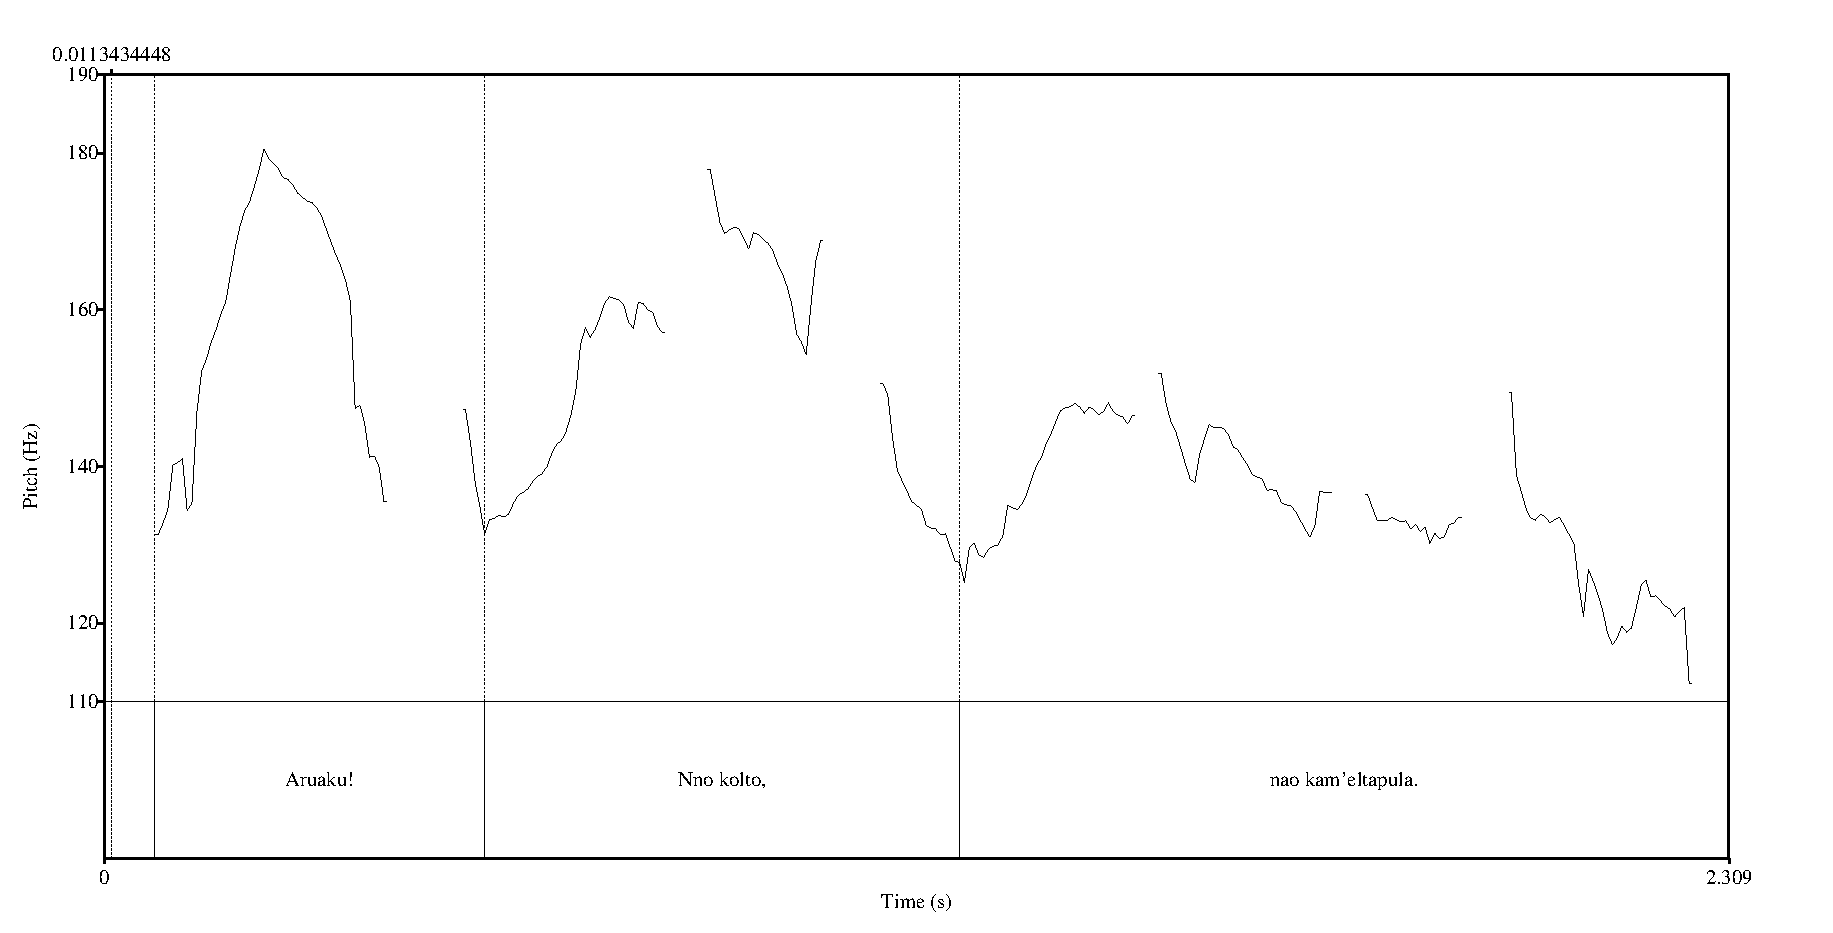
\includegraphics[width=4.8in]{figures/guerinFig1.eps}}
\caption{Intonation contour of example (\ref{Guex:11}) extracted with PRAAT. \label{GuF1}}
\end{figure}



We can now compare (\ref{Guex:11}) and Figure \ref{GuF1} to (\ref{Guex:12ac}) and Figure \ref{GuF2} (from the same story and same male speaker). Example (\ref{Guex:12ac}) contains a \isi{recapitulative linkage}. (\ref{Guex:12a}) is the reference clause, (\ref{Guex:12b}) is the bridging clause, which is juxtaposed (after a pause) to the following clause in (\ref{Guex:12c}). The graph accompanying this example (Fig. \ref{GuF2}) represents the reference and the bridging clauses. It clearly shows that the bridging clause ends on a much higher pitch than the reference clause, which is a \isi{final clause}.


\begin{exe}
\ex \label{Guex:12ac}
\begin{xlist}
\ex \label{Guex:12a}
\gll \underline{Mo-vir}        \underline{sun}   \underline{no-n}          \underline{kou}   \underline{mo-si}. [1.35s]\\
\textsc{3sg}-throw   hat   \textsc{clf-lk}   fowl   \textsc{3sg}-go.down \\
\glt \sqt{He throws down Fowl's hat.}\\
\ex \label{Guex:12b}
\gll \textbf{Mo-vir}      \textbf{sun}    \textbf{no-n}           \textbf{kou}    \textbf{mo-si} [3.4s] \\
\textsc{3sg}-throw   hat   \textsc{clf-lk}   fowl   \textsc{3sg}-go.down\\
\glt \sqt{He throws down Fowl's hat,}\\
\ex \label{Guex:12c}
\gll sun    mo-si          mo-tikel        atano.\\     	       
hat    \textsc{3sg}-go.down   \textsc{3sg}-reach     ground\\
\glt \sqt{the hat goes down onto the ground.} 
\end{xlist}
\end{exe}

\begin{figure}[ht]
\fbox{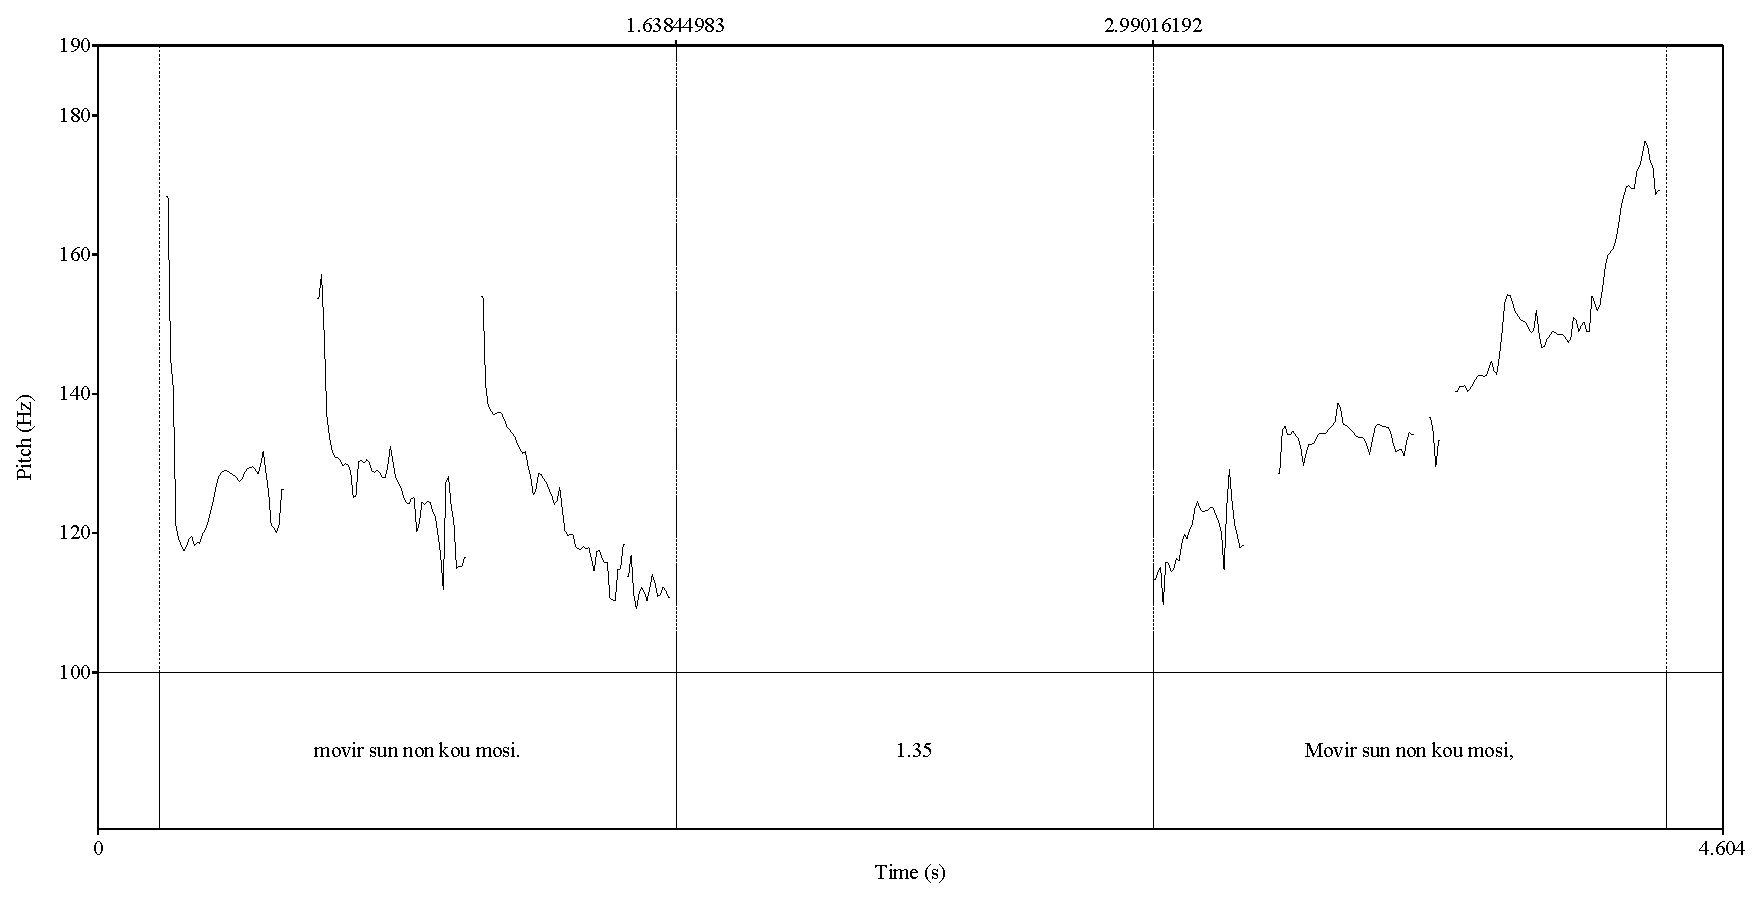
\includegraphics[width=4.8in]{figures/guerinFig2.eps}}
\caption{Intonation contour of examples (\ref{Guex:12a}) and (\ref{Guex:12b}) extracted with PRAAT. \label{GuF2}}
\end{figure}

Example (\ref{Guex:13ac}) also contains a \isi{recapitulative linkage}, but this time, the bridging clause (\ref{Guex:13b}) is overtly \isi{coordinated} to the following clause. All three clauses are represented in Figure \ref{GuF3}. 

\begin{exe}
\ex \label{Guex:13ac}
\begin{xlist}
\ex \label{Guex:13a}
\gll \underline{ko-viris}          \underline{i-si}                 \underline{na}     \underline{kuku}. [1s]\\
\textsc{2sg}-squeeze     \textsc{3sg:irr-}go.down   \textsc{loc}    pot \\
\glt \sqt{You squeeze (out the juice) down into a pot.}\\
\ex \label{Guex:13b}
\gll \textbf{Ko-viris}          \textbf{i-si}               \textbf{na}    \textbf{kuku}   ro [1.09s] \\
\textsc{2sg}-squeeze     \textsc{3sg:irr-}go.down   \textsc{loc}    pot then\\
\glt \sqt{You squeeze (out the juice) down into a pot then,}\\
\ex \label{Guex:13c}
\gll   ko-[0.2s] ku-a.\\     	       
\textsc{2sg}-[pause] boil-\textsc{3sg}\\
\glt \sqt{you...boil it.} 
\end{xlist}
\end{exe}

\begin{figure}[ht]
\fbox{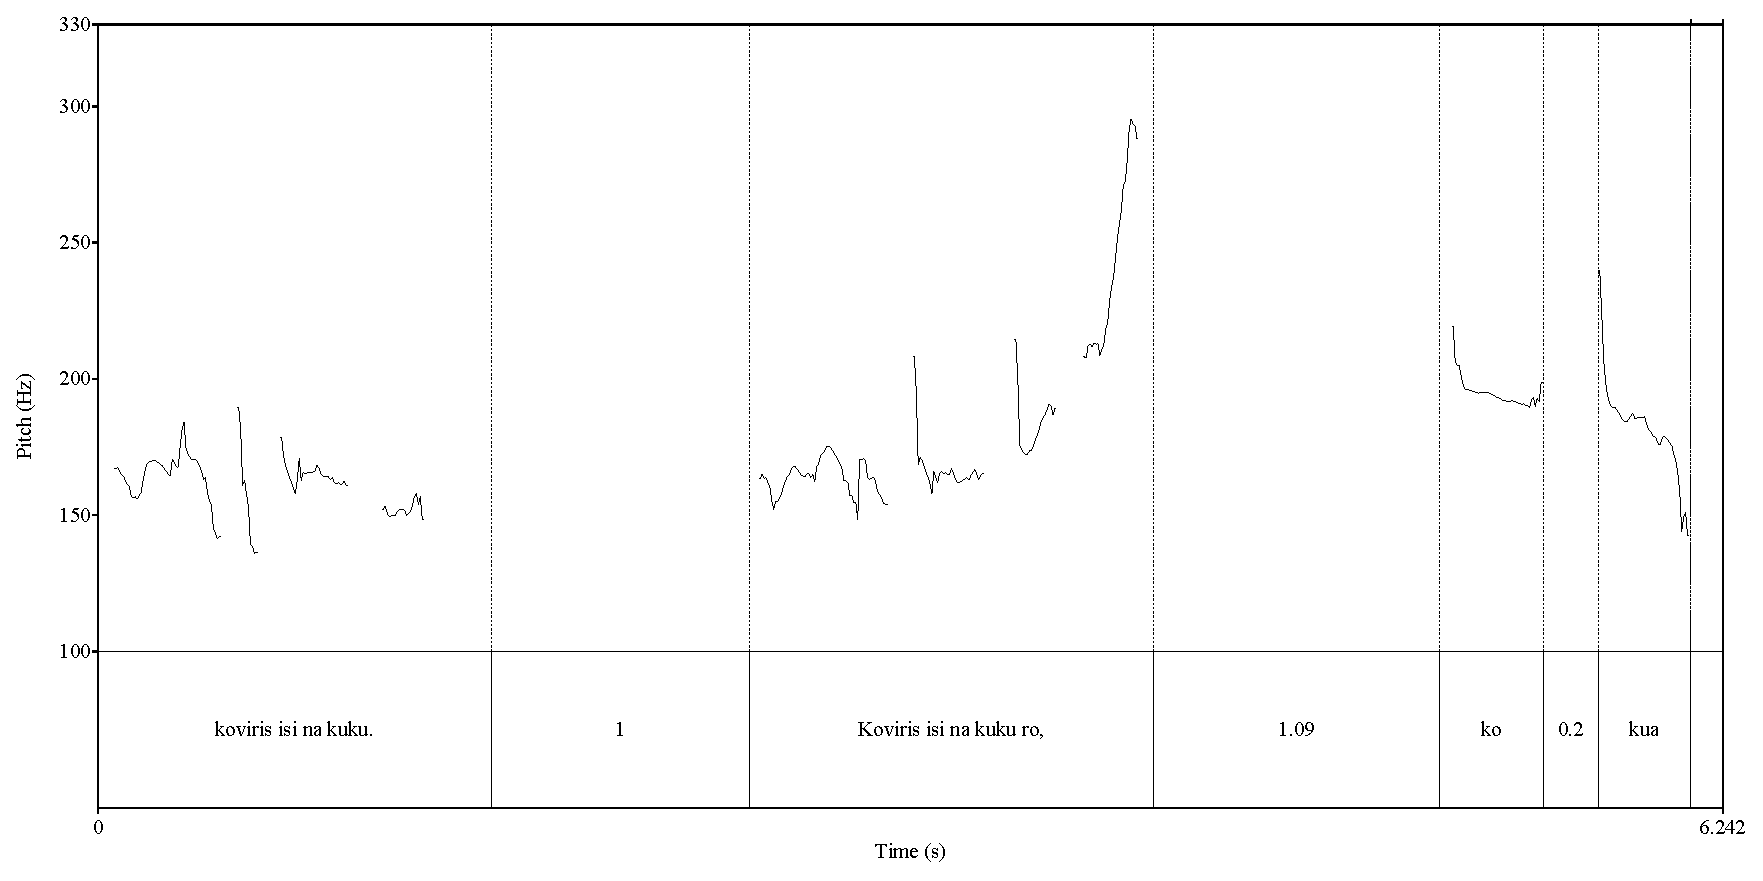
\includegraphics[width=4.8in]{figures/guerinFig3x.eps}}
\caption{Intonation contour of example (\ref{Guex:13ac}) extracted with PRAAT. \label{GuF3}}
\end{figure}

The difference between the bridging clause and the other clauses in (\ref{Guex:13ac}) is visually striking. The reference clause ends with a falling \isi{intonation}. The bridging clause ends on a high pitch with rising \isi{intonation}. The \isi{main clause} following the bridging clause also has falling \isi{intonation}. 

The \isi{intonation} contour of a bridging clause is not always so visually striking. For example, the bridging clause in (\ref{Guex:14b}) shown in  Figure \ref{GuF4} does not rise as much as the one in (\ref{Guex:13b}), although the female speaker is the same in both instances. This is possibly due to the fact that the linkage in (\ref{Guex:14ac}) is a bit unusual: the reference clause is an exclamative clause and not a declarative. There is no pause between the bridging clause and the clause following it. The pitch is much higher throughout. Nevertheless, the bridging clause ends on a pitch higher than the \isi{final clause} preceding it and the \isi{final clause} following it. Based on all examples presented so far, I  extrapolate the fact that although bridging clauses are morphologically main clauses, they indicate continuation and are non-final clauses. Their non-final status is indicated by their \isi{prosody}.


\begin{exe}
\ex \label{Guex:14ac}
\begin{xlist}
\ex \label{Guex:14a}
\gll \underline{\smash{Ko-pos}}          \underline{ko-si}                 \underline{ko-sev!}     [1.11s]\\
\textsc{2sg}-turn    \textsc{2sg}-go.down   \textsc{2sg}-hang \\
\glt \sqt{Turn upside down and hang!}\\
\ex \label{Guex:14b}
\gll \textbf{Ko-pos}          \textbf{ko-si}               \textbf{ko-sev}     ro \\
\textsc{2sg}-turn    \textsc{2sg}-go.down   \textsc{2sg}-hang then\\
\glt \sqt{Turn upside down and hang, then}\\
\ex \label{Guex:14c}
\gll   da-r-sev                  da-r-lala               lang.\\     	       
 \textsc{1pl:incl-du}-hang     \textsc{1pl:incl-du}-take.in   wind\\
\glt \sqt{we both hang [and] enjoy the wind.} 
\end{xlist}
\end{exe}

\begin{figure}[ht]
\fbox{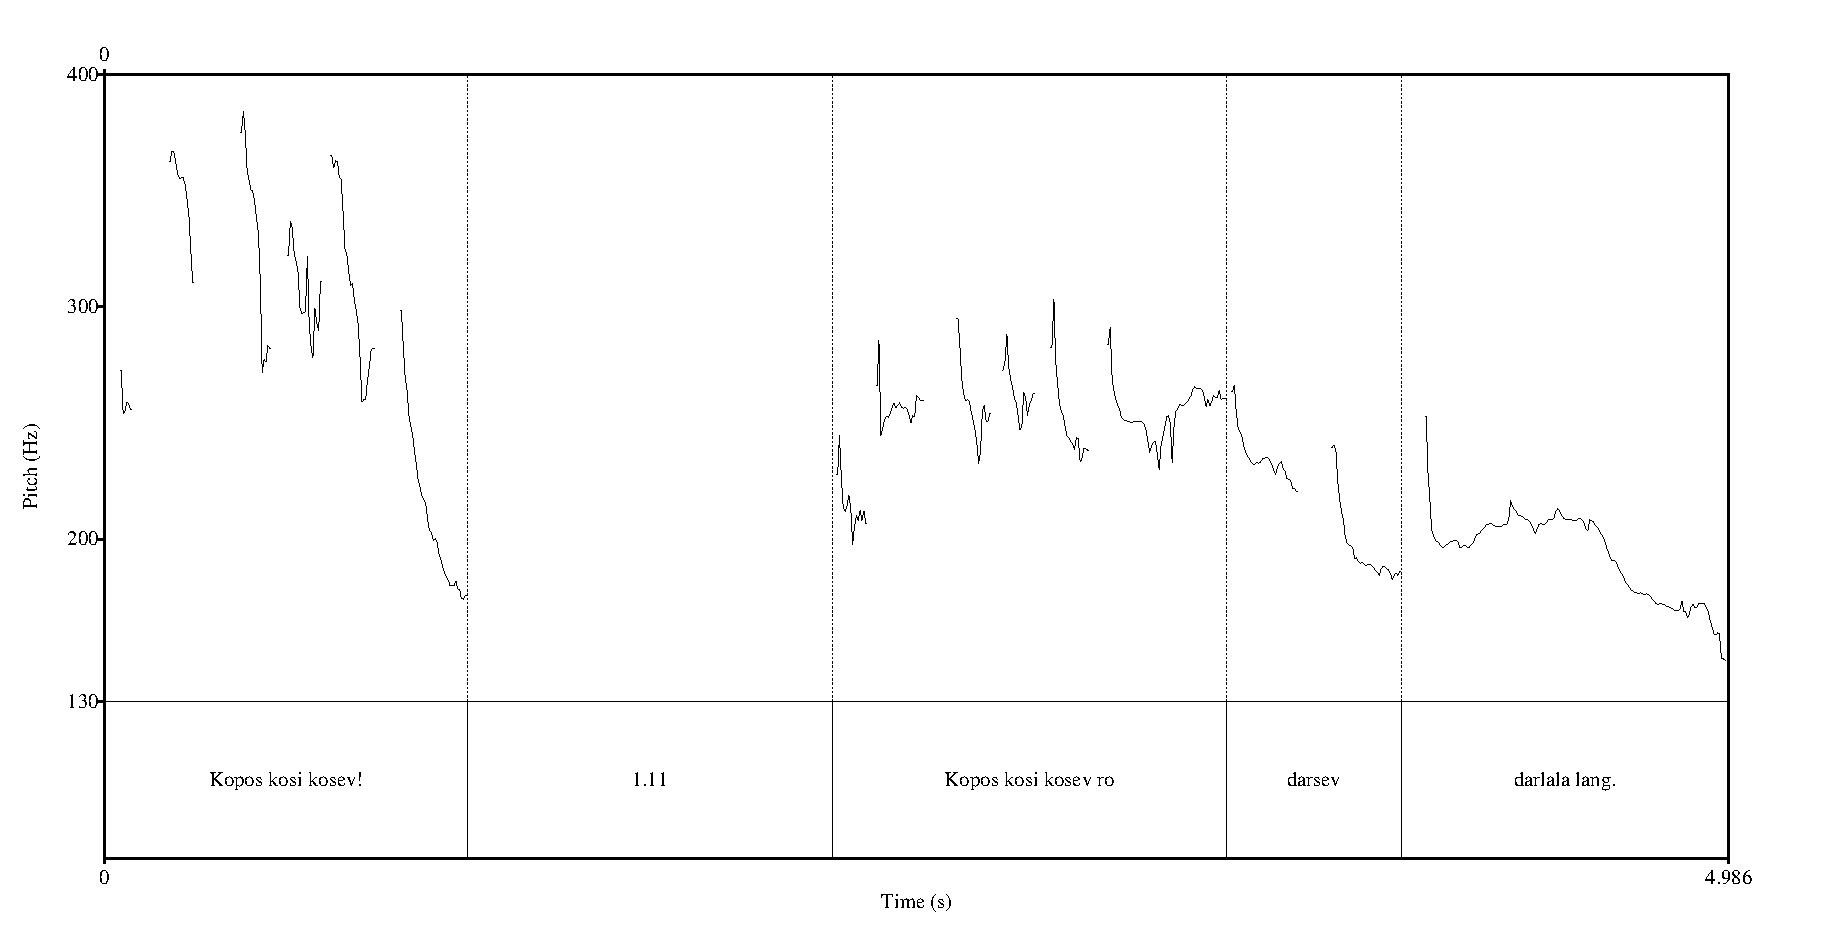
\includegraphics[width=4.8in]{figures/guerinFig4x.eps}}
\caption{Intonation contour of example (\ref{Guex:14ac}) extracted with PRAAT. \label{GuF4}}
\end{figure}

Needless to say, a rising tune is not specific to bridging clauses. When used in paragraph-initial position, time adverbials have a similar \isi{intonation} contour, as shown in Figure \ref{GuF5}, since they too indicate continuation. 

\begin{exe}
\ex \label{Guex:15}
\gll Sur     pong  aite [2.30s]   tina-na                mo-sao.\\     
about   night one      [pause]   mother-\textsc{3sg:poss}   \textsc{3sg}-sick \\
\glt \sqt{One day, his mother was sick.} 
\end{exe}

\begin{figure}[ht]
\fbox{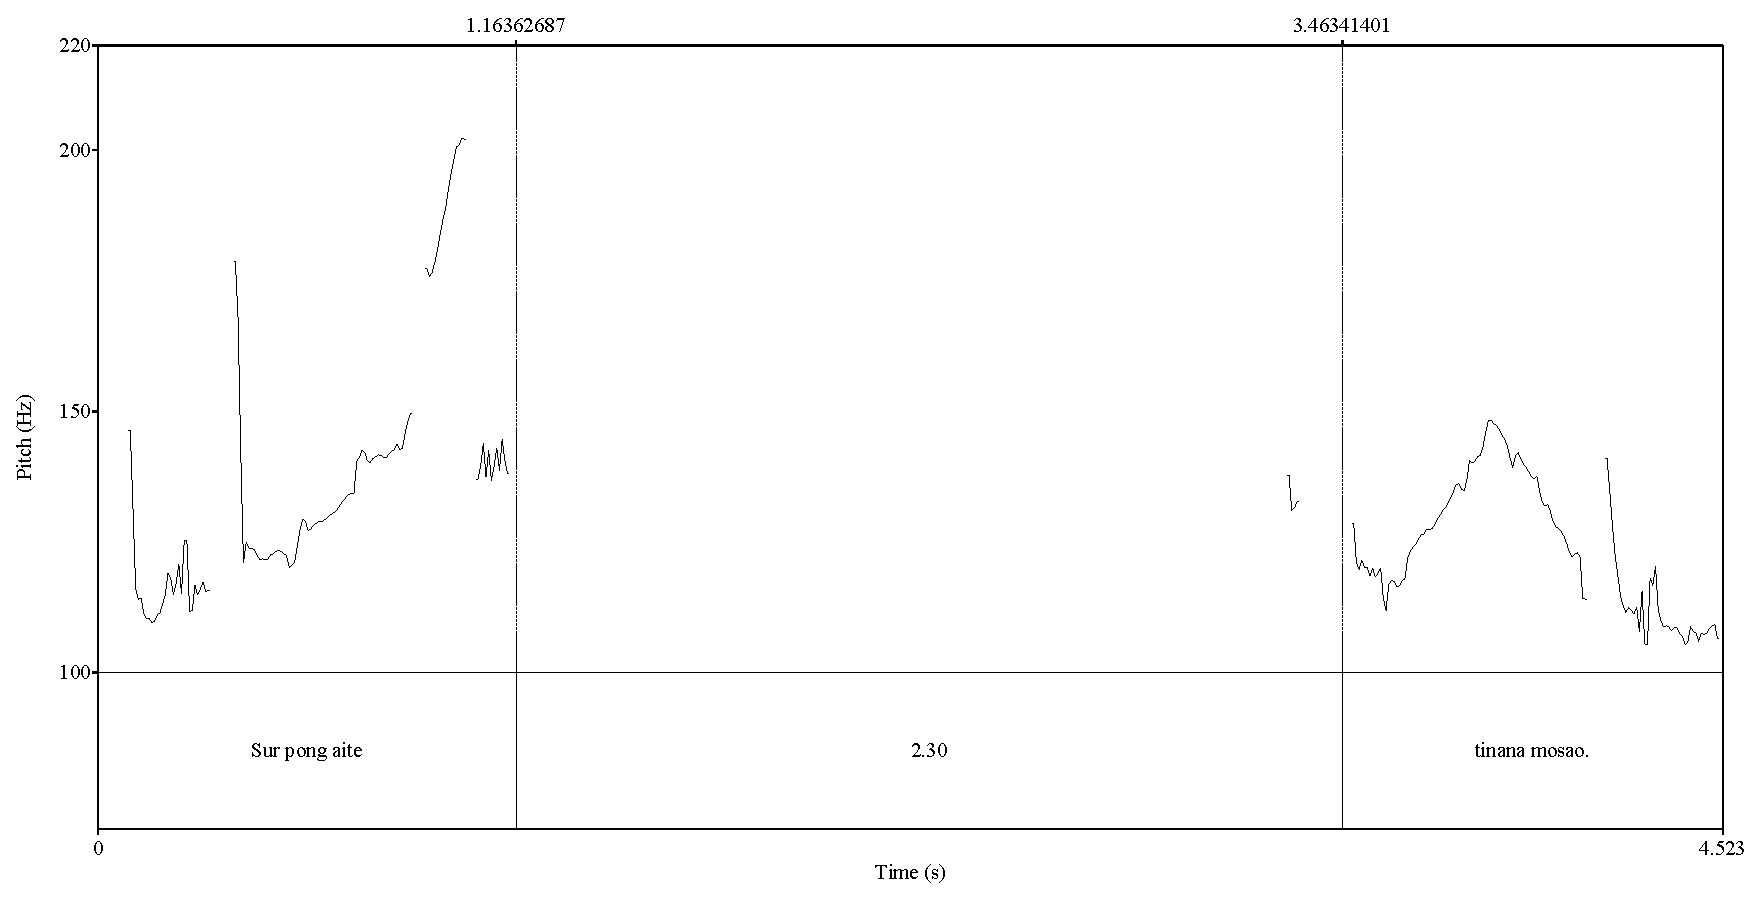
\includegraphics[width=4.8in]{figures/guerinFig5x.eps}}
\caption{Intonation contour of example (\ref{Guex:15}) extracted with PRAAT. \label{GuF5}}
\end{figure}

In addition, clauses which are considered part of a chain of thought and thus non-final also have a rising \isi{intonation} contour, regardless of their morphosyntactic features. This is the case, for example, of lines  (\aREF{Guapp25}) and (\aREF{Guapp26}) of the Appendix, shown in Figure \ref{GuF9}.

\begin{figure}[ht]
\fbox{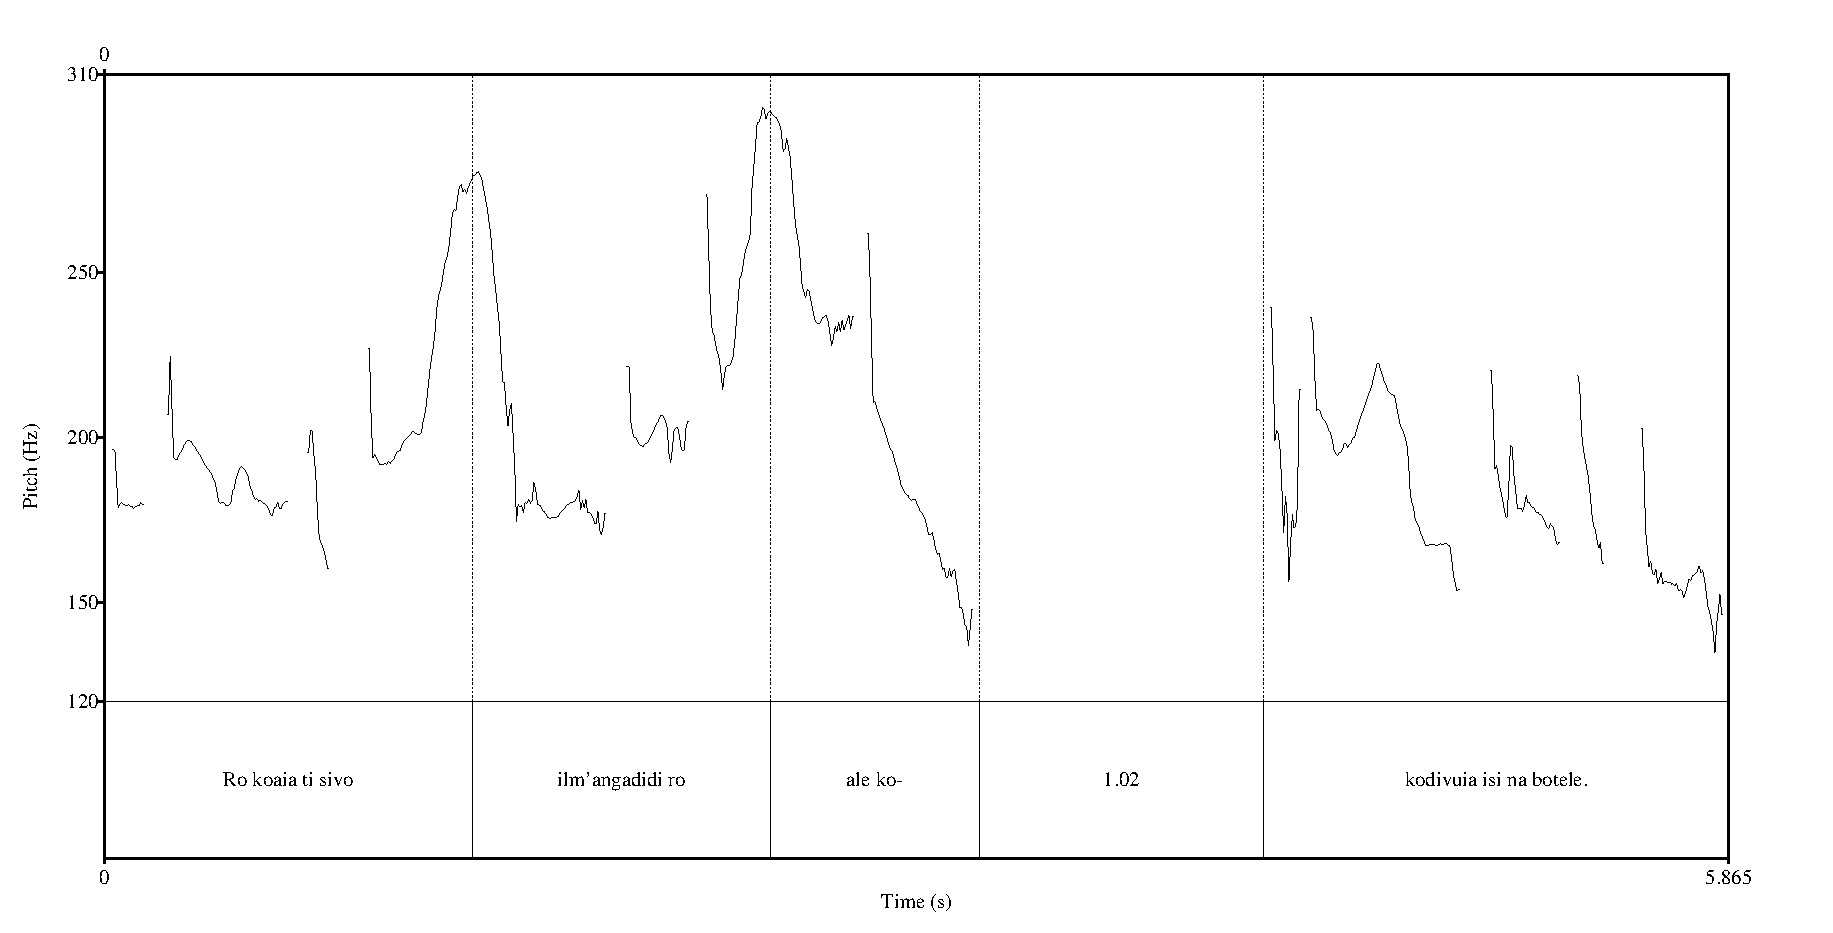
\includegraphics[width=4.8in]{figures/guerinFig9.eps}}
\caption{Intonation contour of examples (\aREF{Guapp25}) and (\aREF{Guapp26}) of the Appendix extracted with PRAAT. \label{GuF9}}
\end{figure}

I have not found so far cases where a clause with rising \isi{intonation} ends a paragraph, a text, or a chain of thoughts, indicating that a rising \isi{intonation} is the preferred contour to expresses continuation in \ili{Mavea} as is the case elsewhere in the \ili{Oceanic} subgroup: in \ili{Manam} \citep[][521]{Lichtenberk83}, in \ili{Paluai} \citep[][63]{Schokkin13}, and in \ili{Abma} \citep[][38]{Schneider10}, to name a few. Final clauses on the other hand have falling \isi{intonation}. 

\section{Bridging constructions in discourse} 
\label{Gusec:Understanding}
Understanding the function of \isi{recapitulative linkage} in discourse rests on two points. First, the discourse genre in which the linkage occurs requires defining given that the function of a bridging construction can vary depending on the \isi{text genre} \citep{devries.2005}. In \refsec{Gusec:frequency}, I present a brief description of \isi{text genres} in \ili{Mavea}. In line with what is reported in the literature (\citealt[][9]{longacre83},  \citealt[][365]{devries.2005}, \citealt[][274]{Thompson.et.al.2007}), \isi{recapitulative linkage} in \ili{Mavea} is most frequent in \isi{narrative} and \isi{procedural texts}.   

Second, the placement of the bridging clause in a particular text is important, as different positions can lead to different meanings. In that respect, I assume that a text evolves into the following stages: exposition, development, developing conflict, climax, denouement, conclusion (as discussed in Chapter 1, this volume). I recognize two major textual components: the \isi{main event line} and the \isi{supporting line} \citep[][14--17]{longacre83} that both help the text progress through the aforementioned stages. To determine the discourse function of \isi{recapitulative linkage} in \ili{Mavea}, I evaluate the clauses immediately surrounding the bridging clause: Does the line preceding the bridging clause report on an event on the main line or the \isi{supporting line}? Is the line following the bridging clause adding new information, i.e., a new event on the main line? Or is it elaborating a previous event, i.e., adding information on the \isi{supporting line}? In \refsec{Gusec:procedural} and \refsec{Gunarrative}, I provide a structural study of two texts in \ili{Mavea} (a \isi{procedural text} and a \isi{narrative}) to determine the placement and function of \isi{recapitulative linkage} in each of these \isi{text genres}. Needless to say, this analysis and the conclusions reached are provisional. More texts of each genre will need to be analyzed before any definite conclusions can be reached.   

\subsection{Text genres and token frequency of recapitulative linkage} 
\label{Gusec:frequency}
Texts are classified based on external criteria such as \isi{topic}, intended audience,
\noindent
purpose, and activity type \citep[][38]{lee01}. In my \ili{Mavea} dataset, I arrive at the following division: 

\begin{itemize}
\item  Conversations: unplanned dialogues between two speakers
\item Anecdotal narratives: personal stories, where the speaker narrates episodes of his/her life
\item Traditional life narratives: depiction (and to some extent explanation) of cultural events and practices such as engagement ceremonies, bride price payment, circumcision, etc.
\item Fiction narratives: stories about fictional protagonists (humans and anthropomorphic characters), sometimes associated with mythical events, which can reveal human nature and sometimes end with a moral lesson. As part of the traditional folklore, these stories are known by everyone in the community.
\item Elicited narratives: invented narratives based on picture books. Participants are given a picture book and asked to invent the story depicted.
\item Procedural texts: elicited texts describing the step-by-step processes to accomplish a task. 
\end{itemize}

To determine the token frequency of \isi{recapitulative linkage} across \isi{text genres}, I formed a corpus in each genre of the same approximate length (around 25 minutes long). The texts were randomly chosen with one exception: there are only six \isi{procedural texts} in my entire dataset (of about 160 recordings). They are all included in the present corpus but they only yield a total of 8 minutes. The results are summarized in Table \ref{GuTable1}.  

\begin{table}[]
\small
\caption{Token frequency of recapitulative linkage per text genre}
\label{GuTable1}
\begin{tabular}{llccc}
\lsptoprule
 \multirow{2}{*}{Text genres} & \multirow{2}{*}{Speakers' data} & Text length, & \# of recap. & Recap.\\
 &                                 & in min.      & linkages  & linkage/min. \\ 
\midrule
Conversations        & 2 \faVenus~age 35--45             & 22                               & 3              & 0.14     \\
Anecdotal narratives & 2 \faMars~age 30--45               & 27                               & 2                                  & 0.07      \\
Traditional life     & {1 \faMars~age 33}                    & {23 }              & {5}                  & {0.22 }        \\
\multirow{2}{*}{Fiction}   & 2 \faMars~, 1 \faVenus              & \multirow{2}{*}{25}                & \multirow{2}{*}{20}    & \multirow{2}{*}{0.8}          \\     
						 & age 33--50                        &                                  &                   &        \\
Elicited narratives  & 4 \faMars~age 25--45               & 24                               & 41                    & 1.71            \\
Procedural texts     & 2 \faVenus~age 45--65             & 8                                & 21                        & 2.63              \\ 
\lspbottomrule
\end{tabular}
\end{table}




Overall, across \isi{text genres}, \isi{recapitulative linkage} is relatively infrequent. A count per minute reveals that it is more frequent in elicited \isi{procedural texts} (2.63 occurrences per minute) and elicited narratives (1.7 occurrences per minute) than in any non-elicited texts (with a maximum of 0.8 occurrences per minute in fiction narratives). It could be that the high count of recapitulative linkages per minute in elicited texts (procedural or \isi{narrative}) gives us indirect evidence that the role of bridging construction is for the speaker to buy (processing) time (\citealt[][378]{devries.2005}; \citeyear[][817]{devries.2006}). As Longacre argues (\citeyear[][9--10]{longacre83}), in many non-literate communities, people learn by participating in activities, rather than being told how to do things in a procedural way. The speakers could be in need of time to think about the procedure in order to retell it or to think of the story to invent, as it was not something they were accustomed to doing. Another interesting point is the fact that bridging clauses are often \isi{coordinated} and followed by a pause (as discussed in \refsec{Gusec:Status}). The speaker can use the \isi{recapitulative linkage} (with continuation \isi{prosody}) and the pause (which occurs after the coordinator \textit{ro} `and, then') to maintain the floor while thinking about the next segment. This could be additional indirect evidence that the speaker buys processing time, as suggested by \citet[][817]{devries.2006}. 


\subsection{Analysis of a procedural text} 
\label{Gusec:procedural}
Procedural texts are goal-oriented texts. They provide a sequence of instructions which are to be closely followed in order to perform a task, to reach a goal. These instructions (which form the \isi{main event line}) are usually temporally ordered and may be interspersed with explanatory material (the \isi{supporting line}), such as elaborations, comments, or advice which provide motivation and justification for the instructions \citep{adam01,fontan08,delpech08}. 

The \isi{procedural text} that I analyze in this section (schematized in Table \ref{GuTable2}) is reproduced in its entirety in the Appendix. Line numbers correspond to the example sentences in the Appendix. The text is a recipe giving instructions on how to make coconut oil. I identify 14 independent events or steps on the main line (mostly \isi{action} verbs) providing instructions and eight events on the \isi{supporting line}, consisting of repetitions (as in line A20) and of elaborations of various sorts (to offer advice (line A7) or provide a refining comment (line A5) on a main line event). 

\begin{table}[]
%\small
\caption{Schema of the recipe: How to make coconut oil}
\label{GuTable2}
\begin{tabular}{lcll}
\textbf{Main line}       & \textbf{Line \#} &   \textbf{Recap. Link.}              & \textbf{Supporting line} \\ \hline
title              & A1     &                 &            \\
purpose         & A2     &                 &                 \\
                & A3     &                 & \isi{repetition} of (A1)      \\
Husk            & A4     &                 &                 \\
                & A5     &                 & \isi{repetition}/elaboration of (4)     \\
Grate           & A6     & reference cl.                &                 \\
                & A7     &                 & elaboration of (A4) and (A5)     \\
                & A8     & bridging cl.  & elaboration     \\
Knead           & A9     &  reference cl.               &                 \\
                & A10     & bridging cl. &                 \\
         & A11     &                 & \isi{repetition} of (A10)/elaboration     \\
Squeeze                & A12     &  reference cl.               &                 \\
                & A13     & bridging cl. &                 \\
Boil            & A14     &                 &                 \\
Put on the fire & A15     & reference cl.                &                 \\
                & A16     &                 & elaboration of (15)   \\
                & A17     &                 & elaboration  of (16)   \\
                & A18     & bridging cl. &                 \\
Stir            & A19     &                 &                 \\
                & A20     &                 & \isi{repetition}  of (A19)    \\
Become oil      & A21     &                 &                 \\
 Stir          & A22     &                &       \\
Hear sizzling   & A23     & reference cl.                  &                 \\
Cooked          & A24     & bridging cl. &                              \\
Remove          & A25     &                 &                 \\
Cool            & A26     &                 &                 \\
Pour            & A27     &                 &                
\end{tabular}
\end{table}

Based solely on the formal characteristics identified in \refsec{Gusec:recapitulative}, I isolate five clear tokens of \isi{recapitulative linkage} in this text. Two instances of \isi{recapitulative linkage}, the pairs (A9--A10) and (A12--A13), are what I consider ``canonical'' examples. In both cases, the reference clauses (lines A9 and A12) are final clauses with falling \isi{intonation}.  The bridging clauses (lines A10 and A13) are \isi{coordinated} to the following clause with \textit{ro} `and'. The bridging clauses are immediately adjacent to the reference clauses and repeat the lexical content verbatim. Both bridging clauses have rising \isi{intonation} contours.\footnote{A reviewer asked why line A11, which I call a \isi{repetition}, was not taken as the bridging clause of line A9. It is indeed possible to envisage a scenario where line A10 is a false start. The speaker starts the bridging clause line A10, changes her mind, and repeats it as line A11 with added  material.}  

The other three recapitulative linkages appear in the pairs (A6--A8), (A15--A18), and (A23--A24). In the first two linkages, (A6--A8) and (A15--A18), the reference and bridging clauses are not immediately adjacent. The \isi{recapitulative linkage} (A6--A8) shows \isi{addition} and \isi{substitution}. The reference clause (line A6) has three consecutive verbs. The first two are separated from the third verb by the coordinator \textit{ro} `and' in the bridging clause (line A8). The first verb of the reference clause is replaced in the bridging clause by a synonym (i.e., \textit{lai} `take' > \textit{la\H{v}i} `take'). The pair (A15--A18) shows \isi{addition} and \isi{omission} in the bridging clause. The pronoun \textit{nna} `it' is added in the bridging clause; the location \textit{na apu} `on the fire', present in the reference clause, is omitted in the bridging clause. Last, the pair (A23--A24) also shows \isi{addition}. The bridging clause contains a more complex predicate: \textit{mov} is a phasal predicate \citep[][342]{guerin11}, added to the predicate of the reference clause \textit{rororo}, an ideophone representing the sound of sizzling food. 

With respect to placement, the bridging clauses in lines A13 and A24 are surrounded by main line events, i.e., new steps in the recipe. The bridging clauses in lines A8 and A18 are preceded by advisory comments on the \isi{supporting line} (lines A7, A16, and A17). They are followed by a new main line event, lines A9 and A19. The reference clause line A9 is preceded by the bridging clause from the previous \isi{recapitulative linkage}. It does not contain a new event per se but an elaboration of the event on the \isi{main event line}, on line A6. The bridging clause line A10 is followed by a \isi{repetition} of itself, line A11, with an added aspectual dimension and continuation \isi{intonation}. 

By looking at the placement of the bridging clauses in the text, we can better deduce their function. The two bridging clauses which appear after material on the \isi{supporting line} (lines A8 and A18) flag a change of orientation, from background to foreground. They bring the \isi{topic} and the audience back onto the \isi{main event line}. On the other hand, the bridging clauses surrounded by main line events (lines A13 and A24) signal that the procedure is continuing. They highlight the \isi{sequentiality} of each step in the recipe and thrust the recipe forward. Recapping one event on the main line (the reference clause) before the next event (in the clause after the bridging clause) ``transform[s] the repeated item from new into given information'' \citep[][224]{brown.2000}.   

The findings are summarized in Table \ref{GuTable3}. It is interesting to note that there are only five clear cases of recapitulative linkages but 14 events on the \isi{main event line} and nine on the \isi{supporting line}, indicating that recapitulative linkages are not obligatory: not all sequences of events are overtly signalled by a bridging clause. 

If speakers have the choice to use or not use a \isi{recapitulative linkage}, we may wonder then what triggers the choice. Events that are not recapped by a bridging clause appear on lines A4, A14, A19, and A24 to A27.  They are followed by repetitions (lines A5, A20), elaboration on the \isi{main event line} (line A15), but they can also continue the procedure. There are new steps (lines \ref{Guapp25} to \ref{Guapp27}) taking place after the end goal of the recipe has been achieved  (line \ref{Guapp24}) but no \isi{recapitulative linkage} to introduce them. Thus, although both the use and non-use of \isi{recapitulative linkage} can conspire to add \isi{thematic continuity}, I conclude that bridging clauses in a \isi{procedural text} either emphasize a temporal semantic relation (e.g., \isi{sequentiality}) or mark an important \isi{narrative} change (back to the \isi{main event line}). 

\begin{table}[]
\scriptsize
\caption{Properties of recapitulative linkage in the procedural text}
\label{GuTable3}
\begin{tabular}{cccccc}
\lsptoprule
\textbf{Line \# of}       & \textbf{Adjacency }  & \textbf{Coordin.}  & \textbf{Recapitu-}   & \textbf{Clauses before/after the} & \textbf{Discourse} \\
\textbf{bridging/}    & \textbf{ bridging/}      & \textbf{or}        & \textbf{lation type}             & \textbf{construction: on }  & \textbf{function}  \\
\textbf{reference } & \textbf{reference} & \textbf{Juxtapos.} & \textbf{}                 & \textbf{main/supporting line}     & \textbf{}          \\
\midrule
\multirow{2}{*}{A6--A8}      & \multirow{2}{*}{no}   & \multirow{2}{*}{juxtaposed }    & \isi{substitution}         & \multirow{2}{*}{supporting/main}    & \multirow{2}{*}{to main event} \\
                          &                            &                   &  and \isi{addition}                &                                 &\\
A9--A10                  & yes                       & \isi{coordinated}        & verbatim                  & main/supporting                   & ?                  \\
A12--A13                  & yes                       & \isi{coordinated}        & verbatim                  & main/main                         & sequencing   \\
\multirow{2}{*}{15--18}  & \multirow{2}{*}{no}    & \multirow{2}{*}{coordinated}        & \isi{omission}      & \multirow{2}{*}{supporting/main}   & \multirow{2}{*}{to main event} \\
                          &                            &                   &  and \isi{addition}                &                                 & \\
A23--A24                  & yes                       & juxtaposed         & \isi{addition}                  & main/main                         & sequencing \\
\lspbottomrule
\end{tabular}
\end{table}

Note also that, in this text, I do not consider the pair A4--A5 to form a \isi{recapitulative linkage}. Although line A5 involves the \isi{repetition} of line A4 with lexical \isi{substitution}, the \isi{intonation} of this pair is the opposite of the \isi{intonation} of a canonical \isi{recapitulative linkage}: line A4 ends with a rising pitch and line A5 a falling pitch. It could be that the speaker is correcting herself. Good coconuts (\textit{\H{m}atiu du}) are old coconuts (\textit{\H{m}atiu patu}), but \textit{\H{m}atiu du} is more of a colloquial term, whereas \textit{\H{m}atiu patu} is the appropriate term for a coconut which has reached maturity. 

In addition, it is unclear at this stage whether the pair A21--A22 forms a \isi{recapitulative linkage} or not.  The second clause (\textit{i-oele} `it is oil') only partially repeats the first clause, which contains a \isi{serial verb construction} (\textit{i-\H{m}a i-oele} `it will become oil'). In comparison, the bridging clauses lines A8, A13, and A18 repeat the entire serial construction in the reference clause. Could it be that line A21 is not a \isi{serial verb construction}? Could it be that \isi{recapitulative linkage} plays a role in differentiating \isi{serial verb construction} from verb juxtaposition? This line of research is left open at this stage.

\subsection{Analysis of a narrative}
\label{Gunarrative}
Narratives are texts that tell a story, imagined or real. Like \isi{procedural texts}, narratives are built on two organizational positions: the \isi{main event line} which carries the plot forward, and the \isi{supporting line} which adds emotive or depictive information. The \isi{narrative} I analyze here (schematized in Table \ref{GuTable4}) is a fiction \isi{narrative} with two anthropomorphized characters: Parrot and Flying Fox. It tells the story of how Parrot tricked Flying Fox into hanging upside down, and how to this day, flying foxes hang upside down. The person narrating this text is the same as the narrator of the \isi{procedural text}.\footnote{I think that it is important to keep in mind the composer of the \isi{narrative} \citep[][17]{longacre83} as bridging constructions are also used as stylistic devices, their usage thus varying along individual preferences. For example, in \ili{Mavea}, I used a picture book to elicit a \isi{narrative}. Two brothers in their early 30s participated. One of the brothers used just one \isi{recapitulative linkage} in his \isi{narrative}, the other more than ten.}

\begin{table}[]
\footnotesize
\caption{Schema of the fiction narrative: Parrot and Flying fox}
\label{GuTable4}
\begin{tabular}{llll}
\textbf{Main line}                             & \textbf{Line \#} &   \textbf{Recap. Link.}      & \textbf{Supporting line}   \\
  Title                                            & 001               &               &               \\
\textbf{Exposition}: information                 & 002--008          &                 &                  \\
about the protagonists.                        &                    &                 &                       \\
They are friends, they live,                     &                   &                 &                          \\
 fly, play, eat together.                       &                    &                 &                             \\
\textbf{Inciting moment}: One day,         & 009--011               &                 &                           \\
they eat. They are satiated.                               &                &                 &                            \\
They sit, they play.                          & 012               &    reference cl.             &                                \\
                                            & 013                 & bridging cl. &                           \\
                                            & 014--017          &                 & \textbf{Background}: Before      \\
                                                 &                   &                 & they were both   \\                          
                                                   &                   &                 & sitting on branches.  \\
                                                &                   &                 & Flying Fox  was not            \\          
                                              &                   &                 & hanging upside down.           \\                                     
\textbf{Inciting moment}: On that day,               & 018               &                 &                                              \\
they eat. They are                                      &                   &                 &                                              \\
satiated, they sit.                    &                   &                 &                                              \\
\textbf{Complicating action}:                         & 019               &                 &                                              \\
Parrot tricks Flying Fox.                      &                   &                 &                                              \\
Parrot hangs upside down.                            & 020               & reference cl.                &                                              \\
                                                 & 021               & bridging cl. &                                              \\
                                                 & 022          &                 & \textbf{Repetition/elaboration}:       \\
                                          &                   &                 & Parrots  hangs               \\
                                            &                   &                 & upside down,               \\                                        
                                                        &                   &                 & he flaps his wings.              \\                                                                      
\textbf{Inciting moment}: Parrot                    & 023          &                 &                                              \\
asks Flying Fox to                        &         024          &  reference cl.               &                                              \\
hang upside down.                         &                   &                 &                                              \\
                                       & 025               & bridging cl. &                                              \\
                                           & 026--027          &                 & \textbf{Repetition/elaboration}:       \\
                                       &                   &                 & They both hang                      \\
                                           &                   &                 & upside down, they play.                      \\                                   
\textbf{Complicating action}:                & 028               &  reference cl.               &                                              \\
Parrot goes back to                  &                   &                 &                                              \\
sitting upright.                       &                   &                 &                                              \\
                                      & 029               & bridging cl. &                                              \\
\textbf{Inciting moment}:                       & 029--031          &                 &                                              \\
Parrot asks Flying Fox                   &                   &                 &                                              \\
to sit upright.                         &                   &                 &                                              \\
\textbf{Climax}: Flying Fox tries                  & 032               &                 &                                              \\
but cannot sit upright,                 &                   &                 &                                              \\
she hangs upside down.                  & 033               &   reference cl.              & \textbf{Repetition}: She keeps         \\
                                            &              &                 &  trying in vain.        \\
\textbf{Denouement}: Flying Fox                   & 034               & bridging cl. &                                              \\
hangs upside down for good.                   &                   &                 &                                              \\
                                               & 035               &                 & \textbf{Summary}:  Parrot tricked                     \\
                                                 &                   &                 & Flying Fox. To this day,                  \\
                                              &                   &                 &  flying foxes hang       \\
                                              &                   &                 &        upside   down.                  \\ 
\end{tabular}
\end{table}



There are 13 events on the main line, and five events on the \isi{supporting line}. I identify four clear cases of \isi{recapitulative linkage}, lines 012--013  shown in (\ref{Guex:17ac}); 020--021 reproduced in (\ref{Guex:18ac}); 024--025 in (\ref{Guex:14ac}); and 028--029 in (\ref{Guex:19ac}). One pair of sentences is ambiguous between a \isi{recapitulative linkage} and a \isi{repetition} (lines 014--015) and is left out of the analysis.  The bridging clauses are all \isi{coordinated} to the following clause using \textit{ro} `and, then'.  The bridging clauses repeat the lexical content of the reference clause verbatim in two cases (012--013; 024--025) while in the other two instances (020--021; 028--029), only the subject noun phrase of the reference clause is not repeated in the bridging clause. All four bridging clauses have rising \isi{intonation} contour and all four reference clauses have falling pitch. Last, all four bridging clauses are immediately adjacent to the reference clauses. 

The end of the \isi{narrative} contains an interesting case which I treat as a \isi{recapitulative linkage} (lines 033--034), despite its unconventional feature. The reference clause in (\ref{Guex:16a}) does not have the typical falling \isi{intonation} of other reference clauses (although it is a \isi{final clause}) because it is  an exclamative clause, marked with a very high pitch. The bridging clause in (\ref{Guex:16b}) has rising \isi{intonation}, as is expected of this type of clause, as shown in Figure \ref{GuF6}.

\begin{exe}
\ex \label{Guex:16ab}
\begin{xlist}
\ex \label{Guex:16a}
\gll \underline{Mo-dere}          \underline{ro},                 \underline{mo-sev!}     [0.87s]\\
\textsc{3sg}-no     then  \textsc{3sg}-hang \\
\glt \sqt{No, she is hanging!}\\
\ex \label{Guex:16b}
\gll  \textbf{Mo-sev}       ro mo-sev         val   \H{v}aite.\\     	       
 \textsc{3sg}-hang   then   \textsc{3sg}-hang     go    once\\
\glt \sqt{She is hanging, then she hangs once and for all.} 
\end{xlist}
\end{exe}

\begin{figure}[ht]
\fbox{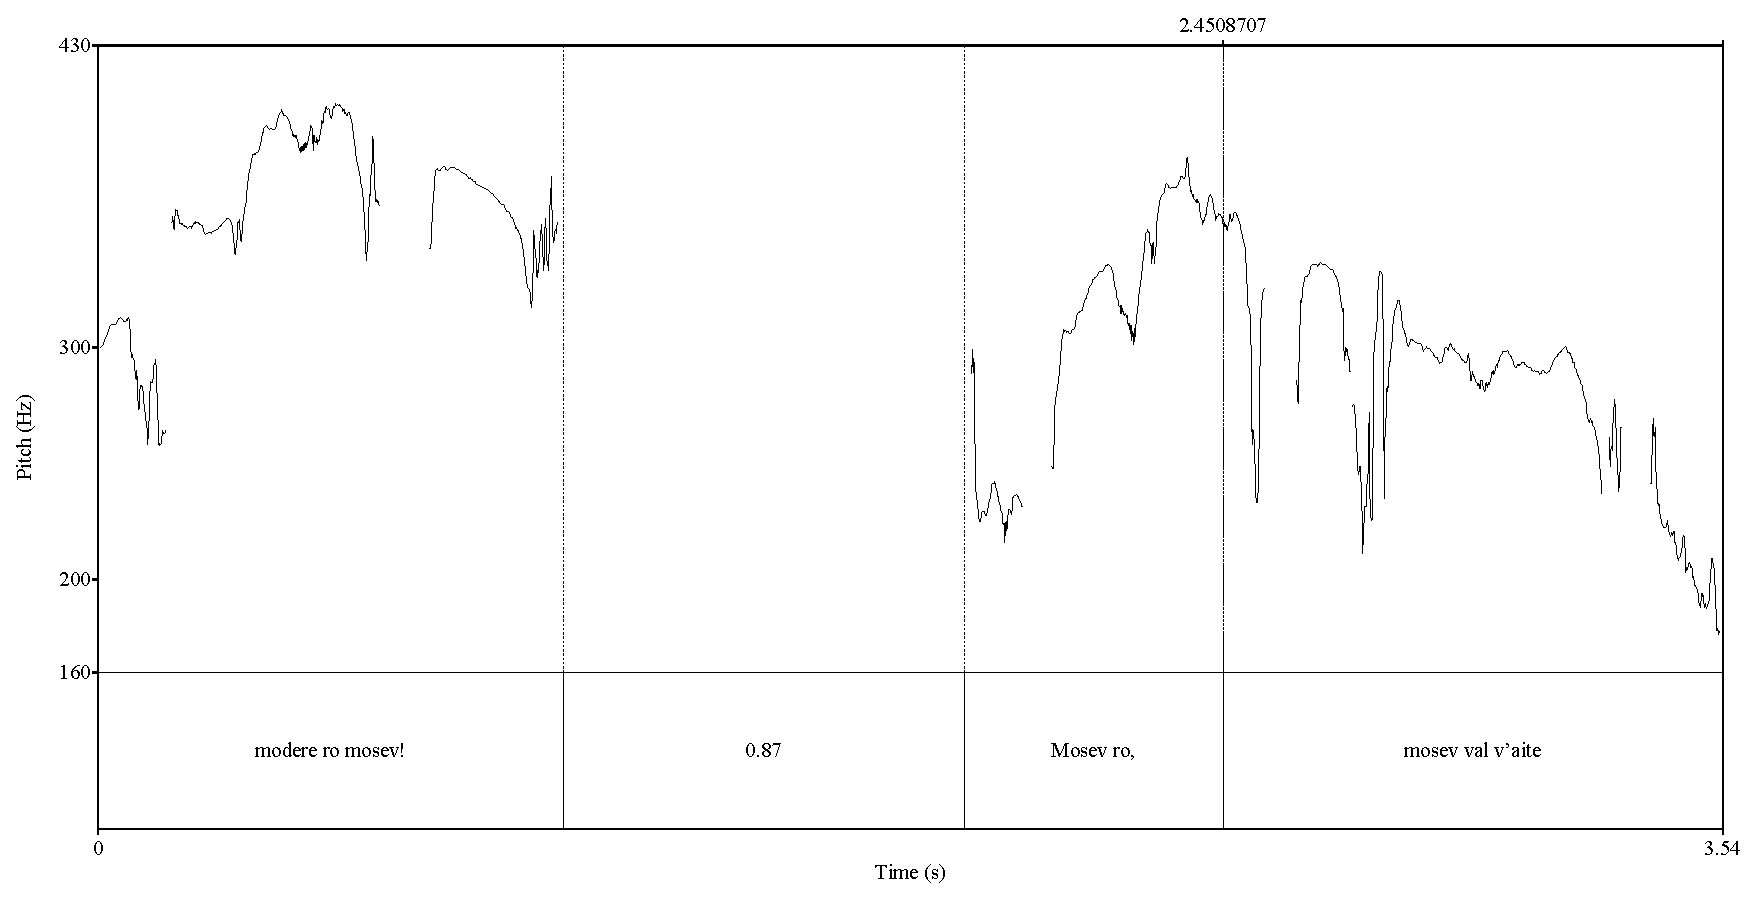
\includegraphics[width=4.8in]{figures/guerinFig6x.eps}}
\caption{Intonation contour of example (\ref{Guex:16ab}) extracted with PRAAT. \label{GuF6}}
\end{figure}


In terms of placement and function, the first instance of \isi{recapitulative linkage} (lines 012--013), reported in (\ref{Guex:17ac}), occurs after a short list of descriptive events on the main line. What is interesting is that the following lines 014--017 provide background information about the animals, as an aside. 

\begin{exe}
\ex \label{Guex:17ac}
\begin{xlist}
\ex \label{Guex:17a}
\gll \underline{Ra-r-\H{m}a{\textasciitilde}\H{m}a\H{v}an.}           [0.85s]\\
\textsc{3pl-du-redup}{\textasciitilde}play \\
\glt \sqt{They were playing with each other.}\\
\ex \label{Guex:17b}
\gll \textbf{Ra-r-\H{m}a{\textasciitilde}\H{m}a\H{v}an}              ro [1.07s]\\
\textsc{3pl-du-redup}{\textasciitilde}play   then\\
\glt \sqt{They were playing with each other then,}\\
\ex \label{Guex:17c}
\gll   \H{m}atan     madia ro raruorua ra-r-lo-sakele.\\     	       
 because   first then two.together \textsc{3pl-du-ipfv}-sit\\
\glt \sqt{because before, they were both sitting (on branches).} 
\end{xlist}
\end{exe}

There is a shift in the narration, from the main line to the \isi{supporting line}. The question is to know whether this is an instance of \isi{thematic discontinuity}. Just before the reference clause, the speaker is using hesitation markers and pauses, which I take to indicate that she buys time to think of her next story segment. However, the pauses are not longer than elsewhere in the same text. It is possible that she realizes that a piece of information is missing. She goes on to add the missing information after the bridging clause. I cannot ascertain that she used the bridging clause ``deliberately'' to mark a change in orientation. 

The \isi{recapitulative linkage} (lines 020--021), reported in (\ref{Guex:18ac}), occurs at a crucial moment in the story, when Parrot hangs upside down. Many repetitions of the verb \textit{sev} `hang' appear in this passage. It seems safe to say that it is also a function of the linkage to add emphasis. This example is also interesting as it shows how a bridging clause in (\ref{Guex:18b}) can be followed by repetitions and elaborations, with the same \isi{intonation} pattern, as shown in Figure \ref{GuF7}, raising the question of the boundary between the different types of recapitulation.\footnote{A reviewer wondered if the \isi{repetition} and elaboration in (\ref{Guex:18b}) and (\ref{Guex:18c}) could be taken as bridging clauses. This analysis would entail that a reference clause could be followed by several bridging clauses.}

\begin{exe}
\ex \label{Guex:18ac}
\begin{xlist}
\ex \label{Guex:18a}
\gll \underline{Si\H{v}i}  \underline{mo-si}           \underline{mo-sev.}           [0.6s]\\
parrot  \textsc{3sg}-go.down   \textsc{3sg}-hang \\
\glt \sqt{Parrot is hanging upside down.}\\
\ex \label{Guex:18b}
\gll \textbf{Mo-si}          \textbf{mo-sev}       ro              mo-sev       ro\\
\textsc{3sg}-go.down   \textsc{3sg}-hang   then  \textsc{3sg}-hang then\\
\glt \sqt{He is hanging upside down, then he is hanging, then}\\
\ex \label{Guex:18c}
\gll   mo-sev    na     palo-na           mo-\H{m}a        i     rua   ro...\\     	       
\textsc{3sg}-hang  \textsc{loc}    leg-\textsc{3sg:poss}   \textsc{3sg}-come  \textsc{lk}   two   then \\
\glt \sqt{he hangs with both his legs then,...} 
\end{xlist}
\end{exe}

%ex17
\begin{figure}[ht]
\fbox{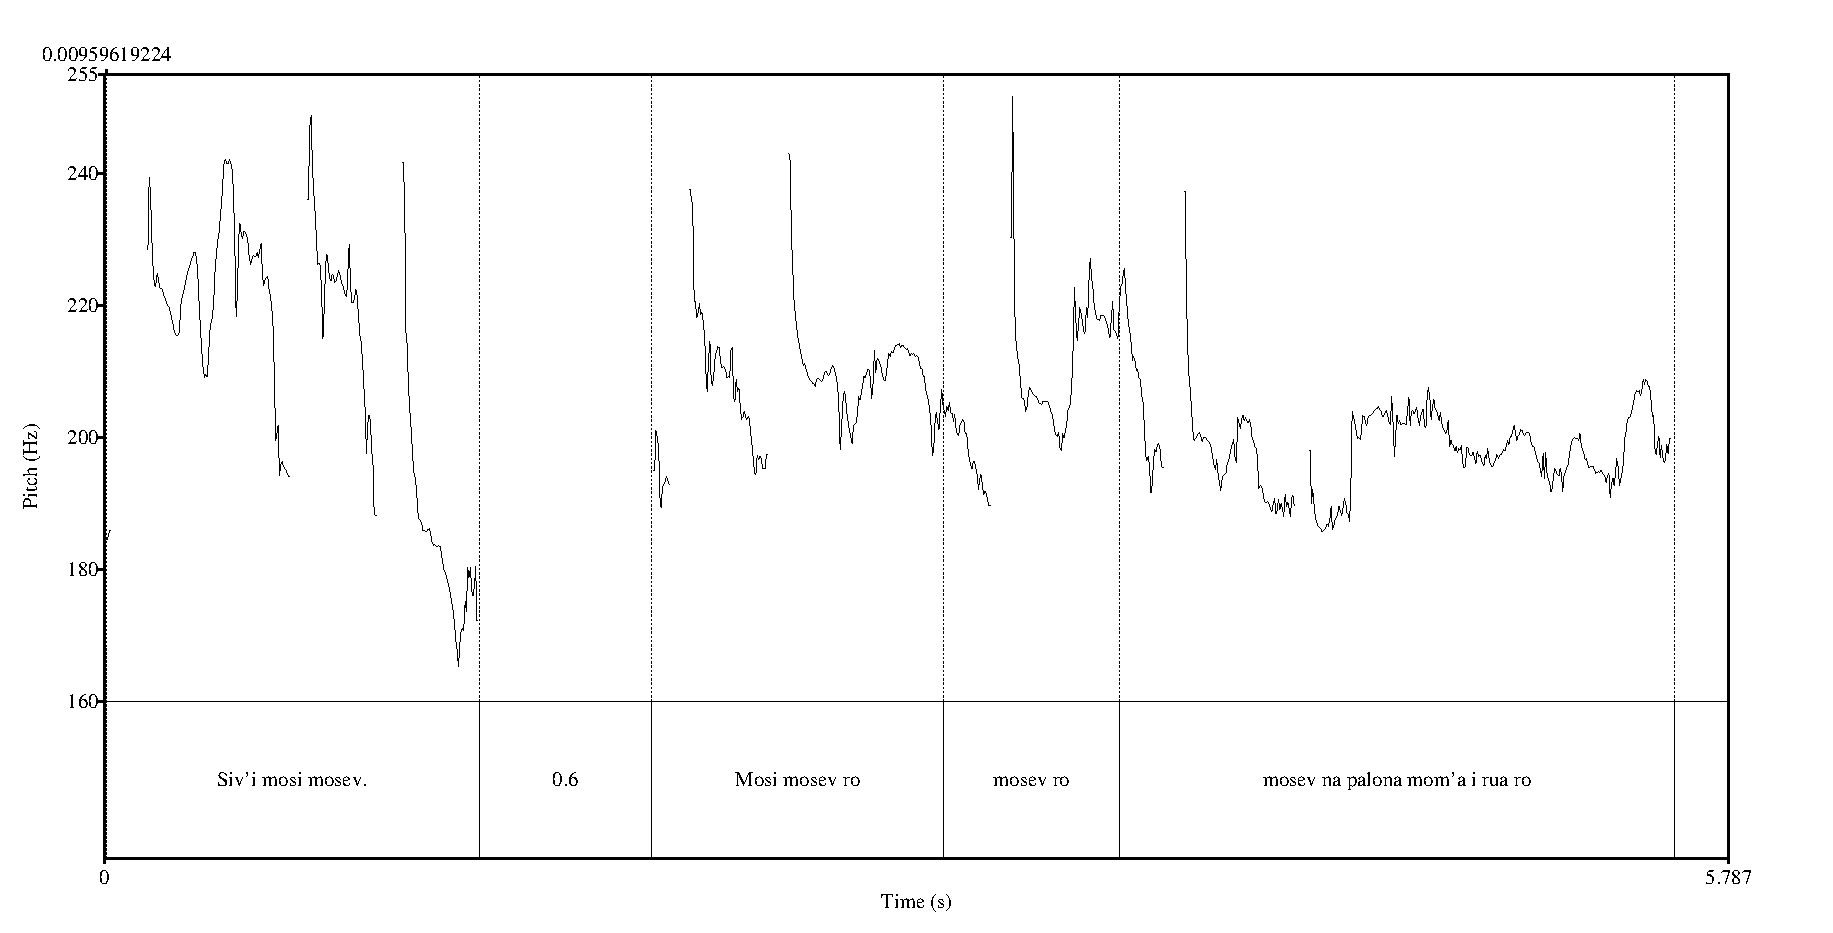
\includegraphics[width=4.8in]{figures/guerinFig7.eps}}
\caption{Intonation contour of example (\ref{Guex:18ac}) extracted with PRAAT. \label{GuF7}}
\end{figure}

The \isi{recapitulative linkage} (lines 024--025) shown in (\ref{Guex:14ac}) is placed inside the direct speech report of Parrot. The reference clause functions as a command, which the bridging clause repeats. This is an important stage in the \isi{narrative} which seals the fate of Flying Fox. The \isi{recapitulative linkage} is interpreted to provide a semantic link between the events (temporal, \isi{sequential}). It also adds emphasis and force to Parrot’s request. 

The next \isi{recapitulative linkage} (028--029) reproduced in (\ref{Guex:19ac}) also highlights an important stage in the \isi{narrative}, the fact that Parrot goes back to his normal sitting position (whereas Flying Fox remains upside down). I interpret this \isi{recapitulative linkage} as functioning like the one before: it adds \isi{sequentiality} but it also underlines this significant turning point in the story.

\begin{exe}
\ex \label{Guex:19ac}
\begin{xlist}
\ex \label{Guex:19a}
\gll \underline{Si\H{v}i}   \underline{\smash{mo-pos}}        \underline{mo-sa}        \underline{mo-sakele}.           [1.49s]\\
parrot   \textsc{3sg}-turn    \textsc{3sg}-go.up   \textsc{3sg}-sit \\
\glt \sqt{Parrot turns back up and sits.}\\
\ex \label{Guex:19b}
\gll \textbf{mo-pos}        \textbf{mo-sa}        \textbf{mo-sakele}          ro [1.07s]\\
\textsc{3sg}-turn    \textsc{3sg}-go.up   \textsc{3sg}-sit   then\\
\glt \sqt{He turns back up and sits, then}\\
\ex \label{Guex:19c}
\gll   mo-tov   karae     mo-v         ``ko-pos!''\\     	       
 \textsc{3sg}-call   flying.fox   \textsc{3sg}-say   \textsc{2sg}-turn\\
\glt \sqt{he calls Flying Fox and says: ``turn!''} 
\end{xlist}
\end{exe}

Last, the denouement of the story is reached. The linkage in the denouement (lines 033--034) is reproduced in (\ref{Guex:16ab}). Again, the bridging clause is followed by an important new stage in the \isi{narrative}: Flying Fox is trapped for good. Here again, the \isi{recapitulative linkage}  is used to highlight this important event. This is also the final point in the \isi{narrative}. The following lines simply summarize the story. 

My analysis appears in Table \ref{GuTable5}. In the \isi{narrative} text, \isi{recapitulative linkage} may have three functions. (i) It adds temporal sequencing and signals that the event following it is new information on the \isi{main event line}. (ii) The bridging clause can announce a shift in orientation between foreground and background.  (iii) In addition, \isi{recapitulative linkage} adds emphasis, or what Longacre calls ``rhetorical underlining''. Around the climactic events, ``the narrator does not want you to miss the important point of the story so he employs extra words at that point'' \citep[][26]{longacre83}. 

\begin{table}[]
\scriptsize
\caption{Properties of recapitulative linkage in the fiction narrative}
\label{GuTable5}
\begin{tabular}{lccccc}
\lsptoprule
\textbf{Line \# of}       & \textbf{Adjacency }  & \textbf{Coordin.}  & \textbf{Recapitu-}   & \textbf{Clauses before/after } & \textbf{Discourse} \\
\textbf{bridging/}    & \textbf{ bridging/}      & \textbf{or}        & \textbf{lation }             & \textbf{the construction: on }  & \textbf{function}  \\
\textbf{reference } & \textbf{reference} & \textbf{Juxtapos.} & \textbf{type}                 & \textbf{  main/supporting }     & \textbf{}          \\
                  &                     &                 & \textbf{}                 &       \textbf{line}     & \textbf{}          \\
\midrule
012--013                  & yes                       & \isi{coordinated}     & verbatim         & main/supporting   & to \isi{supporting line} \\
020--021                  & yes                       & \isi{coordinated}        & \isi{omission}         & main/supporting                   & rhetorical underline        \\
\multirow{2}{*}{024--025 }               & \multirow{2}{*}{yes}                       & \multirow{2}{*}{coordinated}        & \multirow{2}{*}{verbatim }                 & \multirow{2}{*}{main/main}                         & sequencing/ \\
                &                            &                   &               &                                 & rhetorical underline \\
\multirow{2}{*}{028--029}  & \multirow{2}{*}{yes}    & \multirow{2}{*}{coordinated}        & \multirow{2}{*}{omission}      & \multirow{2}{*}{main/main}   & sequencing/  \\
                          &                            &                   &               &                                 & rhetorical underline\\
033--034                  & yes                       & \isi{coordinated}         & verbatim                  & main/main                         & rhetorical underline  \\
\lspbottomrule
\end{tabular}
\end{table}

Comparing the two texts and genres, the data suggest that across \isi{text genres}, a default or unmarked \isi{recapitulative linkage} in \ili{Mavea} (i) is one where the bridging clause repeats the lexical content of the reference clause verbatim with continuation \isi{intonation}; (ii) immediately follows the reference clause; (iii) is overtly \isi{coordinated} to the following clause; and (iv) functions principally as a highlighter. It draws attention to the temporal sequence of events, to the importance of the events (rhetorical underlining), or to shifts in orientation. This shift can be from foreground to background and flag \isi{thematic discontinuity} or the other way around, from background to foreground, and mark \isi{thematic continuity}, bringing the focus back to the (foregrounded) main sequence of events. 

Event sequencing is the most widely acknowledged discourse function of bridging constructions (\citealt[][130, 242, 261]{hasan76};  \citealt[][370]{devries.2005}; \citealt[][273]{Thompson.et.al.2007}). In \ili{Oceanic} languages, it is found in \ili{Nahavaq} \citep[][259]{dimock09}, \ili{Lolovoli} \citep[427]{hyslop01}, \ili{Abma} \citep[24--26]{Schneider09}. Whether event sequencing is a function of the \isi{recapitulative linkage} in \ili{Mavea}, or of the fact that the bridging clause is usually \isi{coordinated} to the following discourse (and \isi{coordination} carries overtones of temporal sequencing), or whether event sequencing is a combination of both strategies requires a more fine-grained analysis \citep[see also][325]{guerin11}. It seems to me that temporal succession is not just a function of the \isi{coordination} strategies. The \isi{conjunction} \textit{(me)ke} in Ughele \citep[][242]{Frostad2012}, \textit{ro} in \ili{Mavea} \citep[][322]{guerin11} and \textit{en} in \ili{Nahavaq} \citep[][230--231]{dimock09} indicate that the conjoined clauses occur simultaneously or in \isi{sequential} order. Similarly, asyndetic \isi{coordination} can denote simultaneity or sequencing (\citealt[][241]{Frostad2012}, \citealt[][425--426]{hyslop01}). A bridging clause, however, does not seem to express simultaneity in \ili{Mavea}. 


\section{Recapitulative linkage versus clausal repetition}
\label{Gurepetition}
Both clausal \isi{repetition} and bridging constructions are common in \ili{Mavea} discourse, and both repeat a verb phrase or a clause previously mentioned. Both can be \isi{coordinated} or juxtaposed to the following clause. How can we tease apart these two constructions?  First, there seems to be an obvious formal distinction between \isi{repetition} and \isi{recapitulative linkage}: the sheer number of repetitions that occur together. Recapitulative linkage involves the \isi{repetition} of the reference clause just once. In verbal repetitions, on the other hand, the verb or clause can be reiterated three or four times, as in (\ref{Guex:20}), and up to eight times in Tuvaluan \citep[][487]{besnier00}.


\begin{exe}
\ex \label{Guex:20}
\gll    \textbf{Mo-tang}     \textbf{mo-tang}   \textbf{mo-tang} mo-lo-\H{v}a.\\     	       
 \textsc{3sg}-cry    \textsc{3sg}-cry  \textsc{3sg}-cry  \textsc{3sg-ipfv}-go\\
\glt \sqt{He cried and cried and kept crying for a while.} \citep[][266]{guerin11}
\end{exe}


Second, verbal \isi{repetition} denotes continuous or iterative events. In many \ili{Ocea\-nic} languages, \isi{repetition} (and \isi{reduplication}) has grammaticalized to express aspectual dimensions such as habitual, imperfective, or iterative (\citealt[][487]{besnier00}; \citealt[][117]{guerin11}; \citealt[][260]{dimock09}). Recapitulative linkage, on the other hand, operates on the level of discourse, marking event completion and temporal sequencing, as discussed in §3. Last, \isi{repetition} and bridging clauses differ in their intonations.  Compare  the \isi{repetition} in (\ref{Guex:21ad}) shown in Figure \ref{GuF8} with the \isi{recapitulative linkage} in Figure \ref{GuF3}, from the same speaker extracted from the same \isi{procedural text} in the Appendix. It is  visually clear that the patterns are very different. The bridging clause in (\ref{Guex:13b}) has a sharp rising pitch, whereas the repetitions in (\ref{Guex:21b}) have a rather flat contour or a falling \isi{intonation}.

\begin{exe}
\ex \label{Guex:21ad}
\begin{xlist}
\ex \label{Guex:21a}
\gll Ko-l-arvulesi-a. [0.88s]       \\
\textsc{2sg-ipfv-}stir-\textsc{3sg}      \\
\glt \sqt{You stir it.}\\
\ex \label{Guex:21b}
\gll \textbf{Ko-arvulesi},   \textbf{ko-arvulesi}, \textbf{ko-arvulesi} pelmel    \\
 \textsc{2sg-}stir \textsc{2sg-}stir \textsc{2sg-}stir  like.this \\
\glt \sqt{You stir, stir,  stir like this, }\\
\ex \label{Guex:21c}
\gll   i-tikel              ma...  [0.82s] \\
   \textsc{3sg}:\textsc{irr}-reach     \textsc{comp} \\
\glt \sqt{until...}\\
\ex \label{Guex:21d}
\gll   i-\H{m}a        i-oele.\\     	       
 \textsc{3sg}:\textsc{irr}-come     \textsc{3sg}:\textsc{irr}-oil\\
\glt \sqt{it becomes oil.} 
\end{xlist}
\end{exe}


\begin{figure}[ht]
\fbox{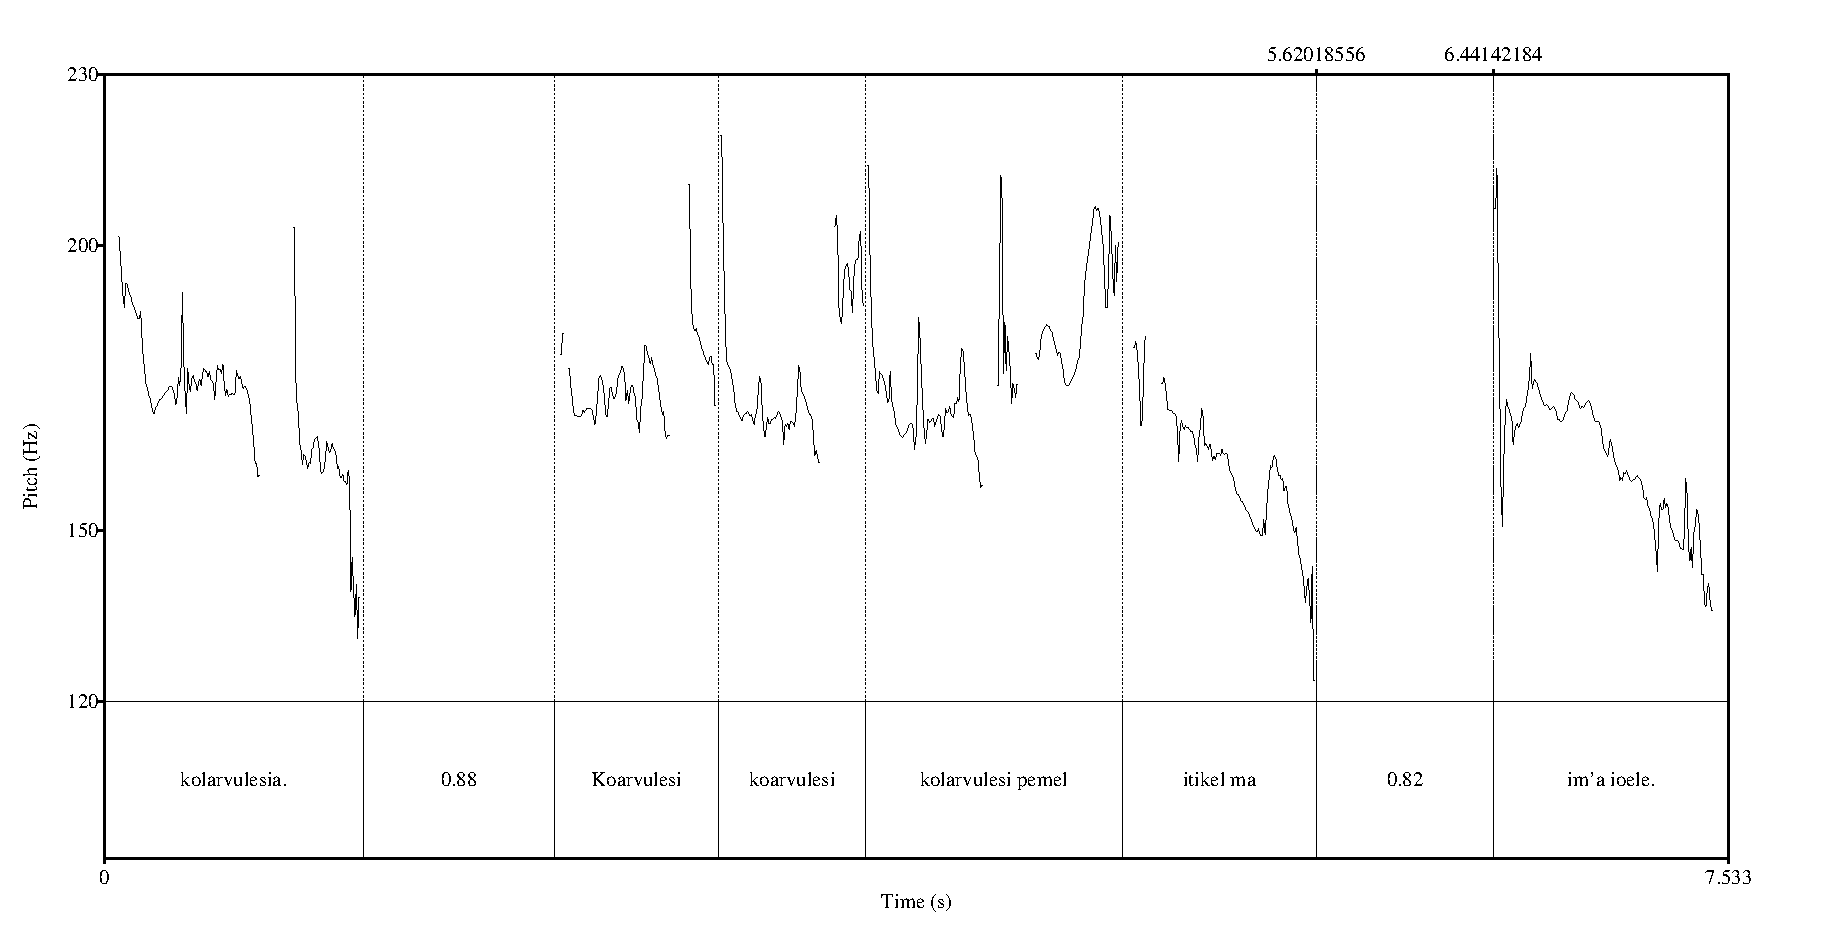
\includegraphics[width=4.8in]{figures/guerinFig8.eps}}
\caption{Intonation contour of example (\ref{Guex:21ad}) extracted with PRAAT. \label{GuF8}}
\end{figure}




\section{Conclusions}
\label{Guconclu}
This chapter  revealed that \isi{recapitulative linkage} in \ili{Mavea} are made up of a final reference clause and a bridging clause which is syntactically a \isi{main clause}, has non-final \isi{prosody}, and is juxtaposed or overtly \isi{coordinated} to a following clause. A similar set of features characterizes \isi{recapitulative linkage} in other languages of Vanuatu (\citealt[][24--26]{Schneider09}; \citealt[][327]{Thieberger06}; \citealt[][426]{hyslop01}) and elsewhere in the \ili{Oceanic} language family (\citealt{palmer09,Frostad2012}; \citealt[][172]{hamel88}; \citealt[][115--116]{Schokkin14}; \citealt[][94]{Lithgow95}). 

A reviewer wonders whether the kind of recapitulation found in \ili{Mavea} can be considered a ``construction'', given that there is no special marker in the grammar and no specific condition triggering obligatory use. The point is well taken; \isi{recapitulative linkage} in \ili{Mavea} is a stylistic feature which has not grammaticalized. However, the lack of apparent form-meaning pairing is also expected if the syntactic profile of a language influences the formal characteristics of bridging constructions in that language (\citealt{devries.2005}; \citealt[][898]{seifart10}). First, in many \ili{Oceanic} languages such as \ili{Sobei}, \ili{Kaulong}, \ili{Roviana} or \ili{Manam} (reported in \citealt{bril10}; \citealt{Lichtenberk83}; \citealt[][53]{lynch02}) \isi{coordination} is preferred over \isi{subordination} as a clause linking strategy.  Therefore, it comes as no surprise that \isi{coordination} is also the preferred strategy for the \isi{recapitulative linkage}. Second, bridging clauses have continuation \isi{intonation}, ending with a rising pitch, which marks them as dependent on the following clause. Even though a rising pitch is by no means a feature peculiar to recapitulative linkages alone, as shown in \refsec{Gusec:Status}, this \isi{prosodic} pattern separates bridging clauses from verbal repetitions. Last, \isi{recapitulative linkage} in \ili{Mavea} is a type of bridging construction given that the pattern has predictable semantic and discourse functions (\refsec{Gusec:Understanding}): to flag thematic (dis)continuity, to add rhetorical underlining, and to highlight temporal succession. Thus, identifying \isi{recapitulative linkage} in \ili{Mavea} requires identifying a constellation of features: syntactic status, \isi{prosodic} contour, semantic relation, and discourse function.

 \section*{Appendix}
 \setcounter{equation}{0}
 \exewidth{(A23)}
Reproduced here is the \isi{procedural text} schematized and analyzed in \refsec{Gusec:procedural}. I had asked the speaker, a woman in her 60s, to explain how to make coconut oil. The arrows at the end of a phrase broadly mark the \isi{intonation} contour. The upper arrow $\uparrow$ indicates that the \isi{intonation} rises, whereas the down arrow $\downarrow$  indicates that the \isi{intonation} falls. No arrow indicates a rather flat \isi{intonation} contour. Pauses in second appear between square brackets.
 
 \begin{exe}
\exi{(A1)} \label{Guapp1}
\gll    Oele-n          \H{m}atiu~$\uparrow$ [0.82s]\\     	       
 oil-\textsc{3sg:poss} coconut [pause]\\
\glt \sqt{Coconut oil,} 
\end{exe}

 \begin{exe}
 \exi{(A2)} \label{Guapp2}
\gll    ko-rong        ko-v       ko-mo-kuk           te      oele~$\downarrow$ [0.6s]\\     	       
\textsc{2sg}-feel     \textsc{2sg}-say   \textsc{2sg-cond}-cook   some    oil [pause]\\
\glt \sqt{suppose  you want to make oil,} 
\end{exe}

  \begin{exe}
\exi{(A3)} \label{Guapp3}
\gll    oele-n          \H{m}atiu~$\uparrow$ [1.31s]\\     	       
 oil-\textsc{3sg:poss} coconut [pause]\\
\glt \sqt{coconut oil,} 
\end{exe}


  \begin{exe}
\exi{(A4)} \label{Guapp4}
\gll    ko-\H{v}a        ko-osom         te      \H{m}ati        du.~$\uparrow$ [1.25s]\\     	       
 \textsc{2sg}-go    \textsc{2sg}-husk      some    coconut   good [pause]\\
\glt \sqt{you husk some good coconuts.} 
\end{exe}


  \begin{exe}
\exi{(A5)} \label{Guapp5}
\gll    Ko-\H{v}a        ko-osom         te      \H{m}ati        patu.~$\downarrow$ [0.7s]\\     	  
 \textsc{2sg}-go    \textsc{2sg}-husk      some    coconut   head [pause]\\
\glt \sqt{You husk some old coconuts.} 
\end{exe}

  \begin{exe}
\exi{(A6)} \label{Guapp6}
\gll    \underline{Ko-lai}      \underline{ko-\H{m}a}~$\uparrow$       \underline{ko-rosi-a}~$\uparrow$ [0.7s]\\     	       
 \textsc{2sg}-take   \textsc{2sg}-come   \textsc{2sg}-grate-\textsc{3sg} [pause]\\
\glt \sqt{You bring them, grate them [i.e., the coconut flesh],} 
\end{exe}


  \begin{exe}
\exi{(A7)} \label{Guapp7}
\gll    ko-mo-osom       i-mo-ngavul                rua   te     i-ngavul    tol, [0.9s]\\     	       
 \textsc{2sg}-\textsc{cond}-husk   \textsc{3sg:irr-cond}-decade   two   or     \textsc{3sg:irr}-decade    three [pause]\\
\glt \sqt{you could husk 20 or 30,} 
\end{exe}

  \begin{exe}
\exi{(A8)} \label{Guapp8}
\gll    \textbf{ko-la\H{v}i}      \textbf{ko-\H{m}a} ro      \textbf{ko-rosi-a}  i-lo-sisi                 na  [0.7s] te dis~$\uparrow$ [0.9s]\\     	       
 \textsc{2sg}-take   \textsc{2sg}-come  and \textsc{2sg}-grate-\textsc{3sg} \textsc{3sg:irr-ipfv}-go.down   \textsc{loc} [pause] some dish [pause]\\
\glt \sqt{you bring them, grate them inside...a dish,} 
\end{exe}

  \begin{exe}
\exi{(A9)} \label{Guapp9}
\gll  i-v             i-mo-ev                  ro~$\uparrow$     \underline{ko-siu-a}.~$\downarrow$  [1.2s]  \\     	       
 \textsc{3sg:irr}-say   \textsc{3sg:irr-cond}-finish   and   \textsc{2sg}-knead-\textsc{3sg}  [pause]\\
\glt \sqt{when [grating] is about done, and you knead it [i.e., the coconut flesh].} 
\end{exe}

  \begin{exe}
\exi{(A10)} \label{Guapp10}
\gll  \textbf{Ko-siu-a}~$\uparrow$  [0.4s] ro [0.2s] \\     	       
\textsc{2sg}-knead-\textsc{3sg} [pause]  and [pause]\\
\glt \sqt{You knead it and} 
\end{exe}


  \begin{exe}
\exi{(A11)} \label{Guapp11}
\gll  \textbf{ko-siu-a} i-lo-\H{v}a                  i-mo-ev                  ro~$\uparrow$   \\     
\textsc{2sg}-knead-\textsc{3sg} \textsc{3sg:irr-ipfv}-go     \textsc{3sg.irr-cond}-finish   and  \\
\glt \sqt{you knead it for a while, and} 
\end{exe}

\begin{exe}
\exi{(A12)} \label{Guapp12}
\gll  ale    \underline{ko-\H{v}iris}          \underline{i-si}                 \underline{na}   \underline{kuku}~$\downarrow$  [1s]\\     	       
then   \textsc{2sg}-squeeze     \textsc{3sg:irr-}go.down   \textsc{loc}  pot  [pause]\\
\glt \sqt{then you squeeze [out the milk] into a cooking pot.} 
\end{exe}

 \begin{exe}
\exi{(A13)} \label{Guapp13}
\gll      \textbf{Ko-\H{v}iris}          \textbf{i-si}                 \textbf{na}   \textbf{kuku} ro~$\uparrow$  [1.09s]\\     	       
   \textsc{2sg}-squeeze     \textsc{3sg:irr-}go.down   \textsc{loc}  pot  and [pause]\\
\glt \sqt{You squeeze [out the milk] into a cooking pot and} 
\end{exe}


  \begin{exe}
\exi{(A14)} \label{Guapp14}
\gll  ko-[0.2s]ku-a.~$\downarrow$  [1.1s]  \\     	       
\textsc{2sg}-[pause]boil-\textsc{3sg} [pause] \\
\glt \sqt{you...boil it.} 
\end{exe}

  \begin{exe}
\exi{(A15)} \label{Guapp15}
\gll  \underline{Ko-ti}       \underline{sa}     \underline{na}  \underline{\smash{apu}}~$\downarrow$  [0.6s]  \\     	       
\textsc{2sg}-put   go.up   \textsc{loc}  fire [pause] \\
\glt \sqt{You put it on the fire.} 
\end{exe}

  \begin{exe}
\exi{(A16)} \label{Guapp16}
\gll  Ko-v      ko-mo-ti          sa      nna   ro $\uparrow$   \\     	       
\textsc{2sg}-say \textsc{2sg-cond}-put   go.up   \textsc{3sg}   and  \\
\glt \sqt{If you put it on [the fire] then} 
\end{exe}

  \begin{exe}
\exi{(A17)} \label{Guapp17}
\gll  ko-sopo-kuro    ti    \H{v}a. $\downarrow$   \\     	       
\textsc{2sg-neg}-leave   put   go  \\
\glt \sqt{don't leave it on.} 
\end{exe}


  \begin{exe}
\exi{(A18)} \label{Guapp18}
\gll  \textbf{Ko-ti}       \textbf{sa}     \textbf{nna}  ro~$\uparrow$  \\     	       
\textsc{2sg}-put   go.up    \textsc{3sg}   and  \\
\glt \sqt{You put it on [the fire],} 
\end{exe}

  \begin{exe}
\exi{(A19)} \label{Guapp19}
\gll  ko-l-arvulesi-a~$\downarrow$  [0.88s]  \\     	       
\textsc{2sg-ipfv}-stir-\textsc{3sg} [pause]\\
\glt \sqt{you stir it.} 
\end{exe}

  \begin{exe}
\exi{(A20)} \label{Guapp20}
\gll  Ko-arvulesi    ko-arvulesi ko-arvulesi   pelmel   \\     	       
\textsc{2sg}-stir \textsc{2sg}-stir \textsc{2sg}-stir like.this \\
\glt \sqt{You stir, stir, stir like this,} 
\end{exe}

  \begin{exe}
\exi{(A21)} \label{Guapp21}
\gll   i-tikel            ma~$\downarrow$     [0.82s]          i-\H{m}a           i-oele.~$\downarrow$ [0.98s]    \\     	       
 \textsc{3sg:irr}-reach     \textsc{comp}    [pause]   \textsc{3sg:irr}-come  \textsc{3sg:irr}-oil [pause]\\
\glt \sqt{until...it becomes oil.} 
\end{exe}

  \begin{exe}
\exi{(A22)} \label{Guapp22}
\gll    I-oele, ko-arvulesi i-lo-\H{v}a \\     	       
  \textsc{3sg:irr}-oil \textsc{2sg}-stir  \textsc{3sg:irr-ipfv}-go\\
\glt \sqt{It [is becoming] oil, you keep stirring} 
\end{exe}

  \begin{exe}
\exi{(A23)} \label{Guapp23}
\gll   ko-rong~$\downarrow$    \underline{sama-na}               \underline{mo-rororo}.     [0.6s] \\ 
 \textsc{2sg}-hear  froth-\textsc{3sg:poss}     \textsc{3sg}-\textsc{ideo}.noise [pause]\\
\glt \sqt{[until] you hear its froth sizzling.} 
\end{exe}

  \begin{exe}
\exi{(A24)} \label{Guapp24}
\gll     \textbf{Sama-na}   mo-v            \textbf{i-rororo}~$\uparrow$    mal  mo-noa         ne~$\downarrow$   [0.88s]   \\     	       
 froth-\textsc{3sg:poss}  \textsc{3sg}-say   \textsc{3sg}-\textsc{ideo}.noise \textsc{dem}  \textsc{3sg}-cooked   \textsc{foc} [pause] \\
\glt \sqt{[When] its froth starts to sizzle, \textsc{it} is cooked.} 
\end{exe}


  \begin{exe}
\exi{(A25)}
\gll     Ro     ko-aia         ti    sivo~$\uparrow$    \\     	       
 and   \textsc{2sg}-remove   put   go.away \\
\glt \sqt{So you remove [it from the fire]} 
\label{Guapp25}
\end{exe}

  \begin{exe}
\exi{(A26)} 
\gll    i-l-\H{m}angadidi               ro~$\uparrow$  \\     	 
 \textsc{3sg:irr-ipfv}-cold        and\\
\glt \sqt{it cools down and} 
\label{Guapp26}
\end{exe}

  \begin{exe}
\exi{(A27)} \label{Guapp27}
\gll   ale    ko-[1.02s]~$\downarrow$      ko-divui-a,  i-si                 na   botele.~$\downarrow$  \\     	       
 then   \textsc{2sg}-[pause]      \textsc{2sg}-pour-\textsc{3sg}  \textsc{3sg:irr}-go.down   \textsc{loc}  bottle\\
\glt \sqt{then, you pour it down into a bottle.} 
\end{exe}



\section*{Abbreviations}
\textsc{:} portmanteau,
\textsc{-} affix boundary,
\textsc{1}		first person,
\textsc{2}		second person,
\textsc{3} 		third person,
\textsc{br}		basic root,
\textsc{cit}		citation root,
\textsc{clf}		classifier,
\textsc{comp}		complementizer,
\textsc{cond}		conditional,
\textsc{det}		determiner,
\textsc{dist.pst}		distant past,
\textsc{du}		dual,
\textsc{excl}		exclusive,
\textsc{foc}		focus marker,
\textsc{ideo}		ideophone,
\textsc{incl}		inclusive,
\textsc{iter}		iterative,
\textsc{lk}		linker,
\textsc{loc}		locative,
\textsc{ipfv}		imperfective,
\textsc{irr} 		irrealis,
\textsc{neg} 		negation,
\textsc{pl} 		plural,
\textsc{poss} 		possessive,
\textsc{pro} 		pronoun,
\textsc{redup} 		reduplicant,
\textsc{sg} 		singular,
\textsc{tr} 		transitive marker




\section*{Acknowledgements}
Sincere thanks to both reviewers whose insightful comments helped improve this chapter, and to my consultants, friends, and families on Mavea Island.
\sloppy

\printbibliography[heading=subbibliography,notkeyword=this] 
\end{document}
